% ===================================================================== %
%  Apresentação de TCC — Ciência da Computação / IC-UFAL
%  João Matheus Nascimento Dias
%
%  Classe: UFAL-beamer-moderno.cls
%  Compilar: latexmk -pdf main   (duas passadas: barra de progresso e
%            total de páginas)
%
%  Estrutura (defesa de 30 min, ~1 slide/min):
%    1. Problema .......... 4 slides   (por que a pergunta importa)
%    2. Fundamentos ....... 4 slides   (só o necessário para ler os gráficos)
%    3. Como medi ......... 5 slides   (o que garante que a comparação é justa)
%    4. Resultados ........ 8 slides   (uma afirmação por slide, no título)
%    5. O que significa ... 4 slides   (a tese do trabalho)
%    6. Fecho ............. 3 slides
%    + backup com os quadros e tabelas oficiais da monografia
% ===================================================================== %
\documentclass{UFAL-beamer-moderno}

\usepackage{booktabs}
\usepackage{tabularx}
\usepackage{siunitx}
\sisetup{output-decimal-marker={,}, group-separator={\,}, mode=text}

% deck autocontido: todas as imagens em img/ (cópias das figuras da monografia)
\graphicspath{{img/}}

% Cores das séries nas figuras do Cap. 4
\definecolor{fwA}{HTML}{2A78D6}
\definecolor{fwB}{HTML}{EB6834}
\newcommand{\A}{\textcolor{fwA}{\textbf{A}}}
\newcommand{\B}{\textcolor{fwB}{\textbf{B}}}
\newcommand{\fwA}{\textcolor{fwA}{\textbf{Firmware A}}}
\newcommand{\fwB}{\textcolor{fwB}{\textbf{Firmware B}}}
\newcommand{\en}[1]{\textit{#1}}   % termo em inglês (\emph da classe é destaque)

% frase-chave centralizada, para fechar um slide
\newcommand{\punch}[1]{%
  \begin{center}\color{ufalNavy}\large\bfseries #1\end{center}}

% --------------------------------------------------- %
%                  Informações                         %
% --------------------------------------------------- %
\doctype{Trabalho de Conclusão de Curso}
\title[Aquisição de sinais digitais com a RP2350]{Uma abordagem hardware/software
para aquisição de sinais digitais com a RP2350}
\author[João Matheus]{João Matheus Nascimento Dias}
\supervisor{Prof. Dr. Erick de Andrade Barboza}
\institute[IC/UFAL]{Instituto de Computação --- Universidade Federal de Alagoas}
\date[Nov/2026]{Maceió, novembro de 2026}
\ufallogo{IC.jpg}

\begin{document}

\titlepage

\begin{frame}{Roteiro}
  \tableofcontents[hideallsubsections]
\end{frame}

% ===================================================================== %
\section{O problema}
% ===================================================================== %

\begin{frame}{Um analisador lógico mede \emph{quando} cada borda aconteceu}
  \begin{columns}[T]
    \begin{column}{0.52\textwidth}
      \begin{itemize}
        \setlength{\itemsep}{8pt}
        \item Grava o estado de vários pinos ao longo do tempo e decodifica
              protocolos (I2C, SPI, UART\ldots)
        \item Versões em microcontrolador custam dezenas de reais e falam com
              o \textbf{sigrok/PulseView}
        \item Tudo depende de uma hipótese: amostras \textbf{igualmente
              espaçadas} e \textbf{nenhuma faltando}
      \end{itemize}
    \end{column}
    \begin{column}{0.44\textwidth}
      \centering
      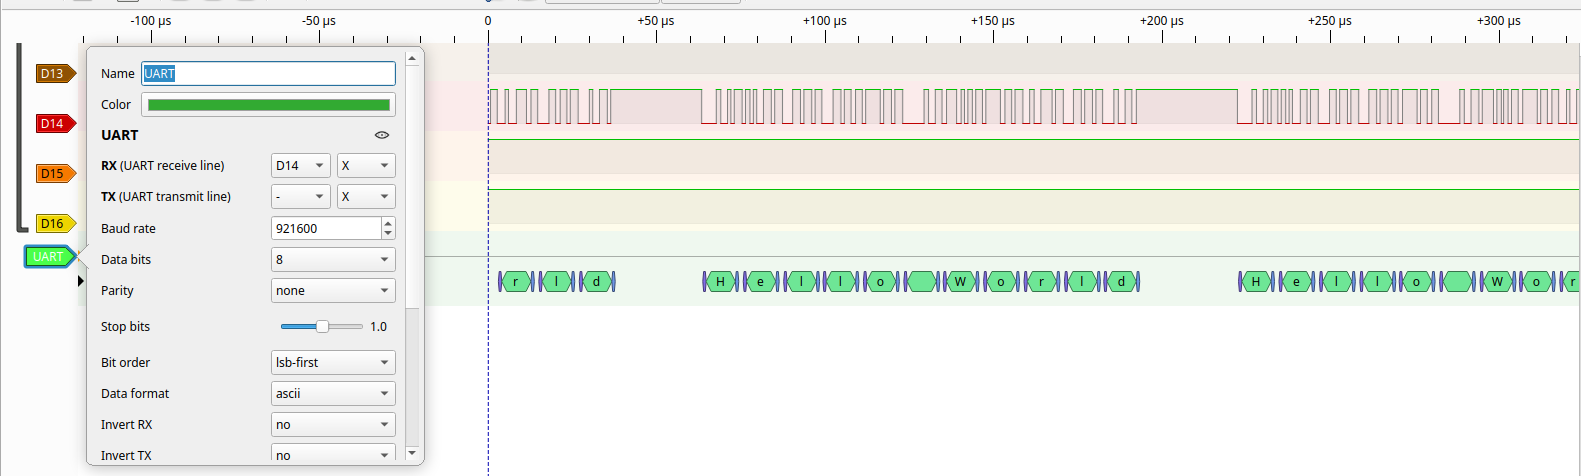
\includegraphics[width=\linewidth]{fig_2_8_pulseview.png}\\[2pt]
      \src{Autoria própria.}
    \end{column}
  \end{columns}
\end{frame}

\begin{frame}{Duas formas de obter a amostra --- no mesmo chip}
  \begin{columns}[T]
    \begin{column}{0.48\textwidth}
      \textcolor{fwB}{\textbf{GPIO+CPU (software)}}
      \begin{itemize}
        \item a própria CPU lê os pinos em um laço e conta o tempo
        \item simples, portável, sem periférico especial
        \item a mesma CPU também comprime e envia pelo USB
      \end{itemize}
      \vspace{6pt}
      \centering
      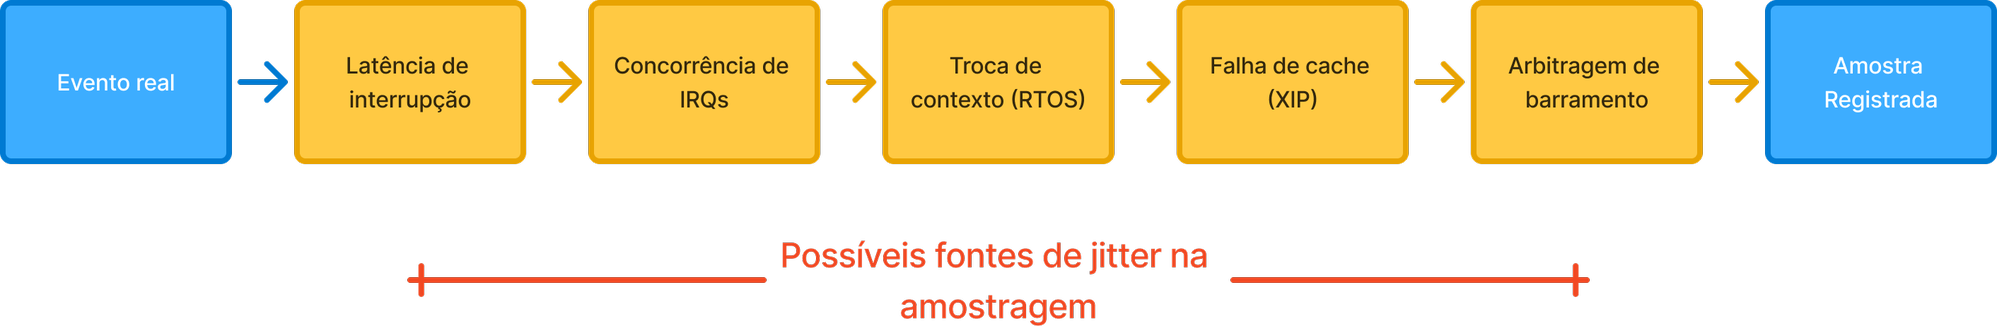
\includegraphics[width=0.94\linewidth]{fig_2_3_nao_determinismo_gpio_cpu.png}
    \end{column}
    \begin{column}{0.48\textwidth}
      \textcolor{fwA}{\textbf{PIO+DMA (hardware)}}
      \begin{itemize}
        \item o \textbf{PIO} amostra sozinho, síncrono ao \en{clock}
        \item a \textbf{DMA} leva as amostras à SRAM sem a CPU
        \item a CPU só comprime e envia
      \end{itemize}
      \vspace{6pt}
      \centering
      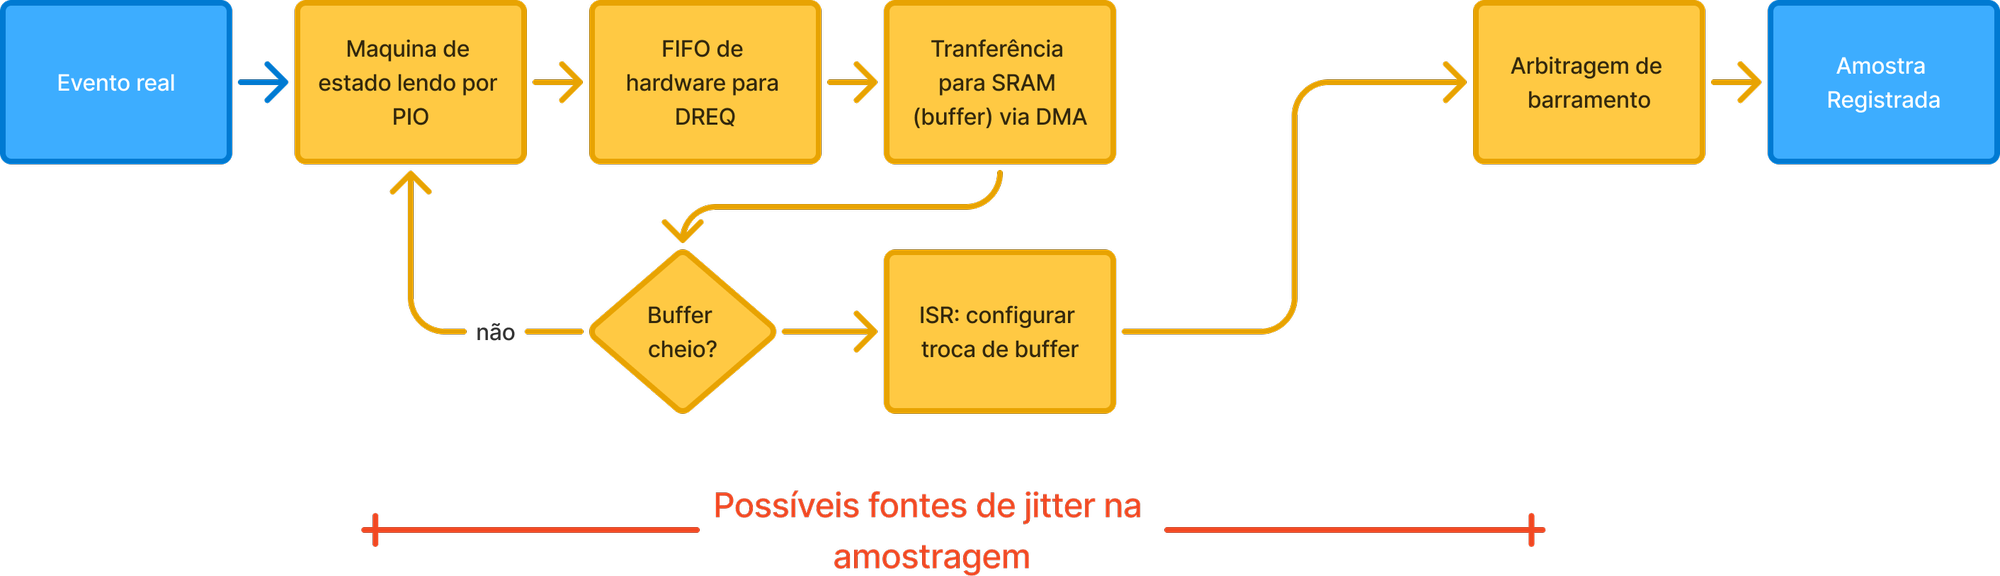
\includegraphics[width=0.94\linewidth]{fig_2_7_nao_determinismo_pio_dma.png}
    \end{column}
  \end{columns}
  \vspace{2pt}
  \centering\src{Autoria própria.}
\end{frame}

\begin{frame}{O argumento é conhecido; a medida, não}
  \notebox{``Laço de software é limitado pelos ciclos por iteração e sofre
  \en{jitter}; um periférico dedicado amostra de forma determinística.''}
  \vspace{6pt}
  \begin{itemize}
    \setlength{\itemsep}{6pt}
    \item A literatura descreve as duas abordagens, mas \textbf{não as mede
          lado a lado}: falta mesma plataforma, mesmo protocolo, mesma pilha
          USB, mesma codificação
    \item Projetos de referência (sigrok-pico) \textbf{assumem} o PIO sem
          quantificar o ganho
  \end{itemize}
  \vspace{10pt}
  \punch{A partir de que taxa a leitura de GPIO pela CPU deixa de bastar\\
  e o PIO+DMA passa a ser indispensável?}
\end{frame}

\begin{frame}{Objetivos}
  \begin{block}{Objetivo geral}
    Avaliar experimentalmente o impacto da arquitetura de aquisição,
    comparando \textbf{PIO+DMA} e \textbf{GPIO+CPU} em um analisador lógico
    embarcado com transmissão contínua via USB.
  \end{block}
  \vspace{8pt}
  \begin{enumerate}
    \setlength{\itemsep}{7pt}
    \item Implementar a arquitetura GPIO+CPU \textbf{no mesmo \en{firmware}},
          preservando protocolo, pilha USB e codificação
    \item Definir e instrumentar quatro métricas: taxa sustentada,
          \en{jitter}, perda em captura contínua e ocupação de CPU
    \item Montar bancada com sinal conhecido, \textbf{referência externa} e
          execução automatizada, com análise estatística definida a priori
  \end{enumerate}
\end{frame}

% ===================================================================== %
\section{Fundamentos}
% ===================================================================== %

\begin{frame}{Amostrar rápido não basta: o intervalo precisa ser constante}
  \begin{columns}[T]
    \begin{column}{0.50\textwidth}
      \centering
      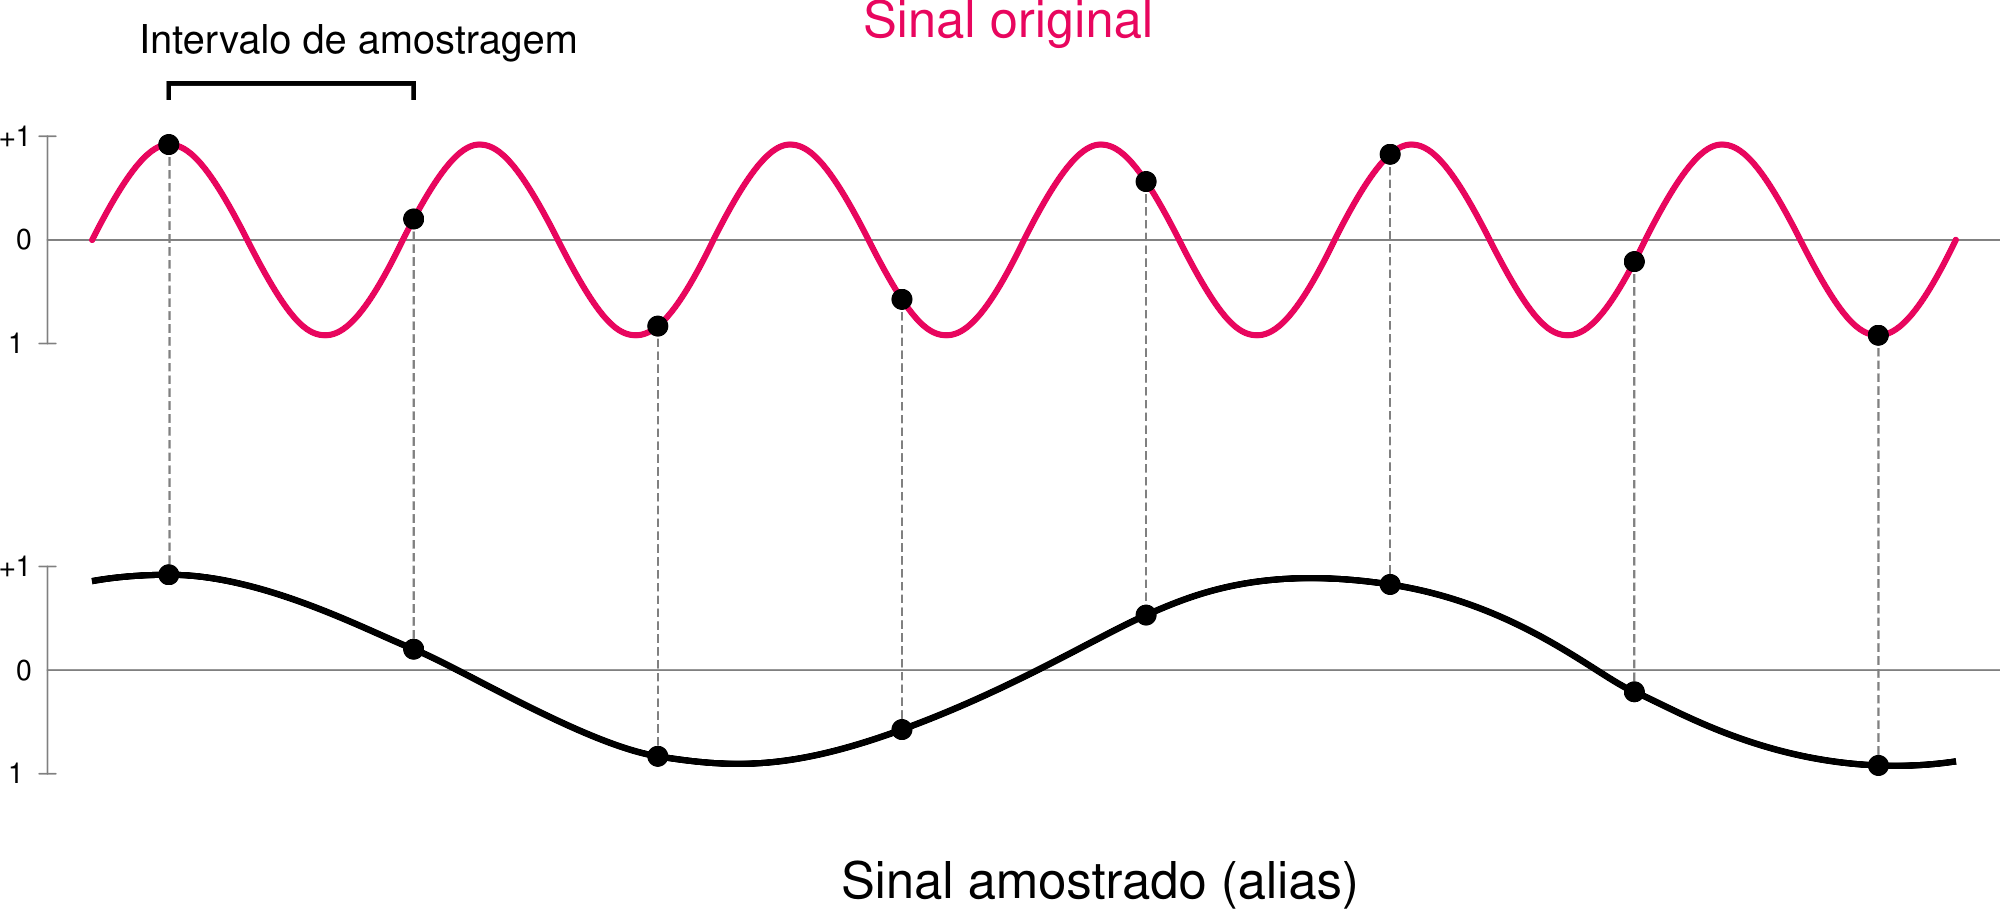
\includegraphics[width=\linewidth]{fig_2_1_aliasing.png}\\[2pt]
      \src{adaptado de Krol, licença CC0.}
    \end{column}
    \begin{column}{0.46\textwidth}
      \begin{itemize}
        \setlength{\itemsep}{6pt}
        \item Nyquist--Shannon: $f_s > 2f_{max}$; abaixo disso há
              \en{aliasing} e a informação se perde
        \item Formas de onda digitais (bordas, pulsos estreitos) exigem na
              prática \textbf{4 a 10$\times$} a fundamental
      \end{itemize}
      \alertbox{Uma amostra tomada tarde desloca a borda medida, e o erro
      \textbf{não se recupera} no pós-processamento.}
    \end{column}
  \end{columns}
\end{frame}

\begin{frame}{Três grandezas descrevem o comportamento temporal}
  \begin{columns}[T]
    \begin{column}{0.50\textwidth}
      \centering
      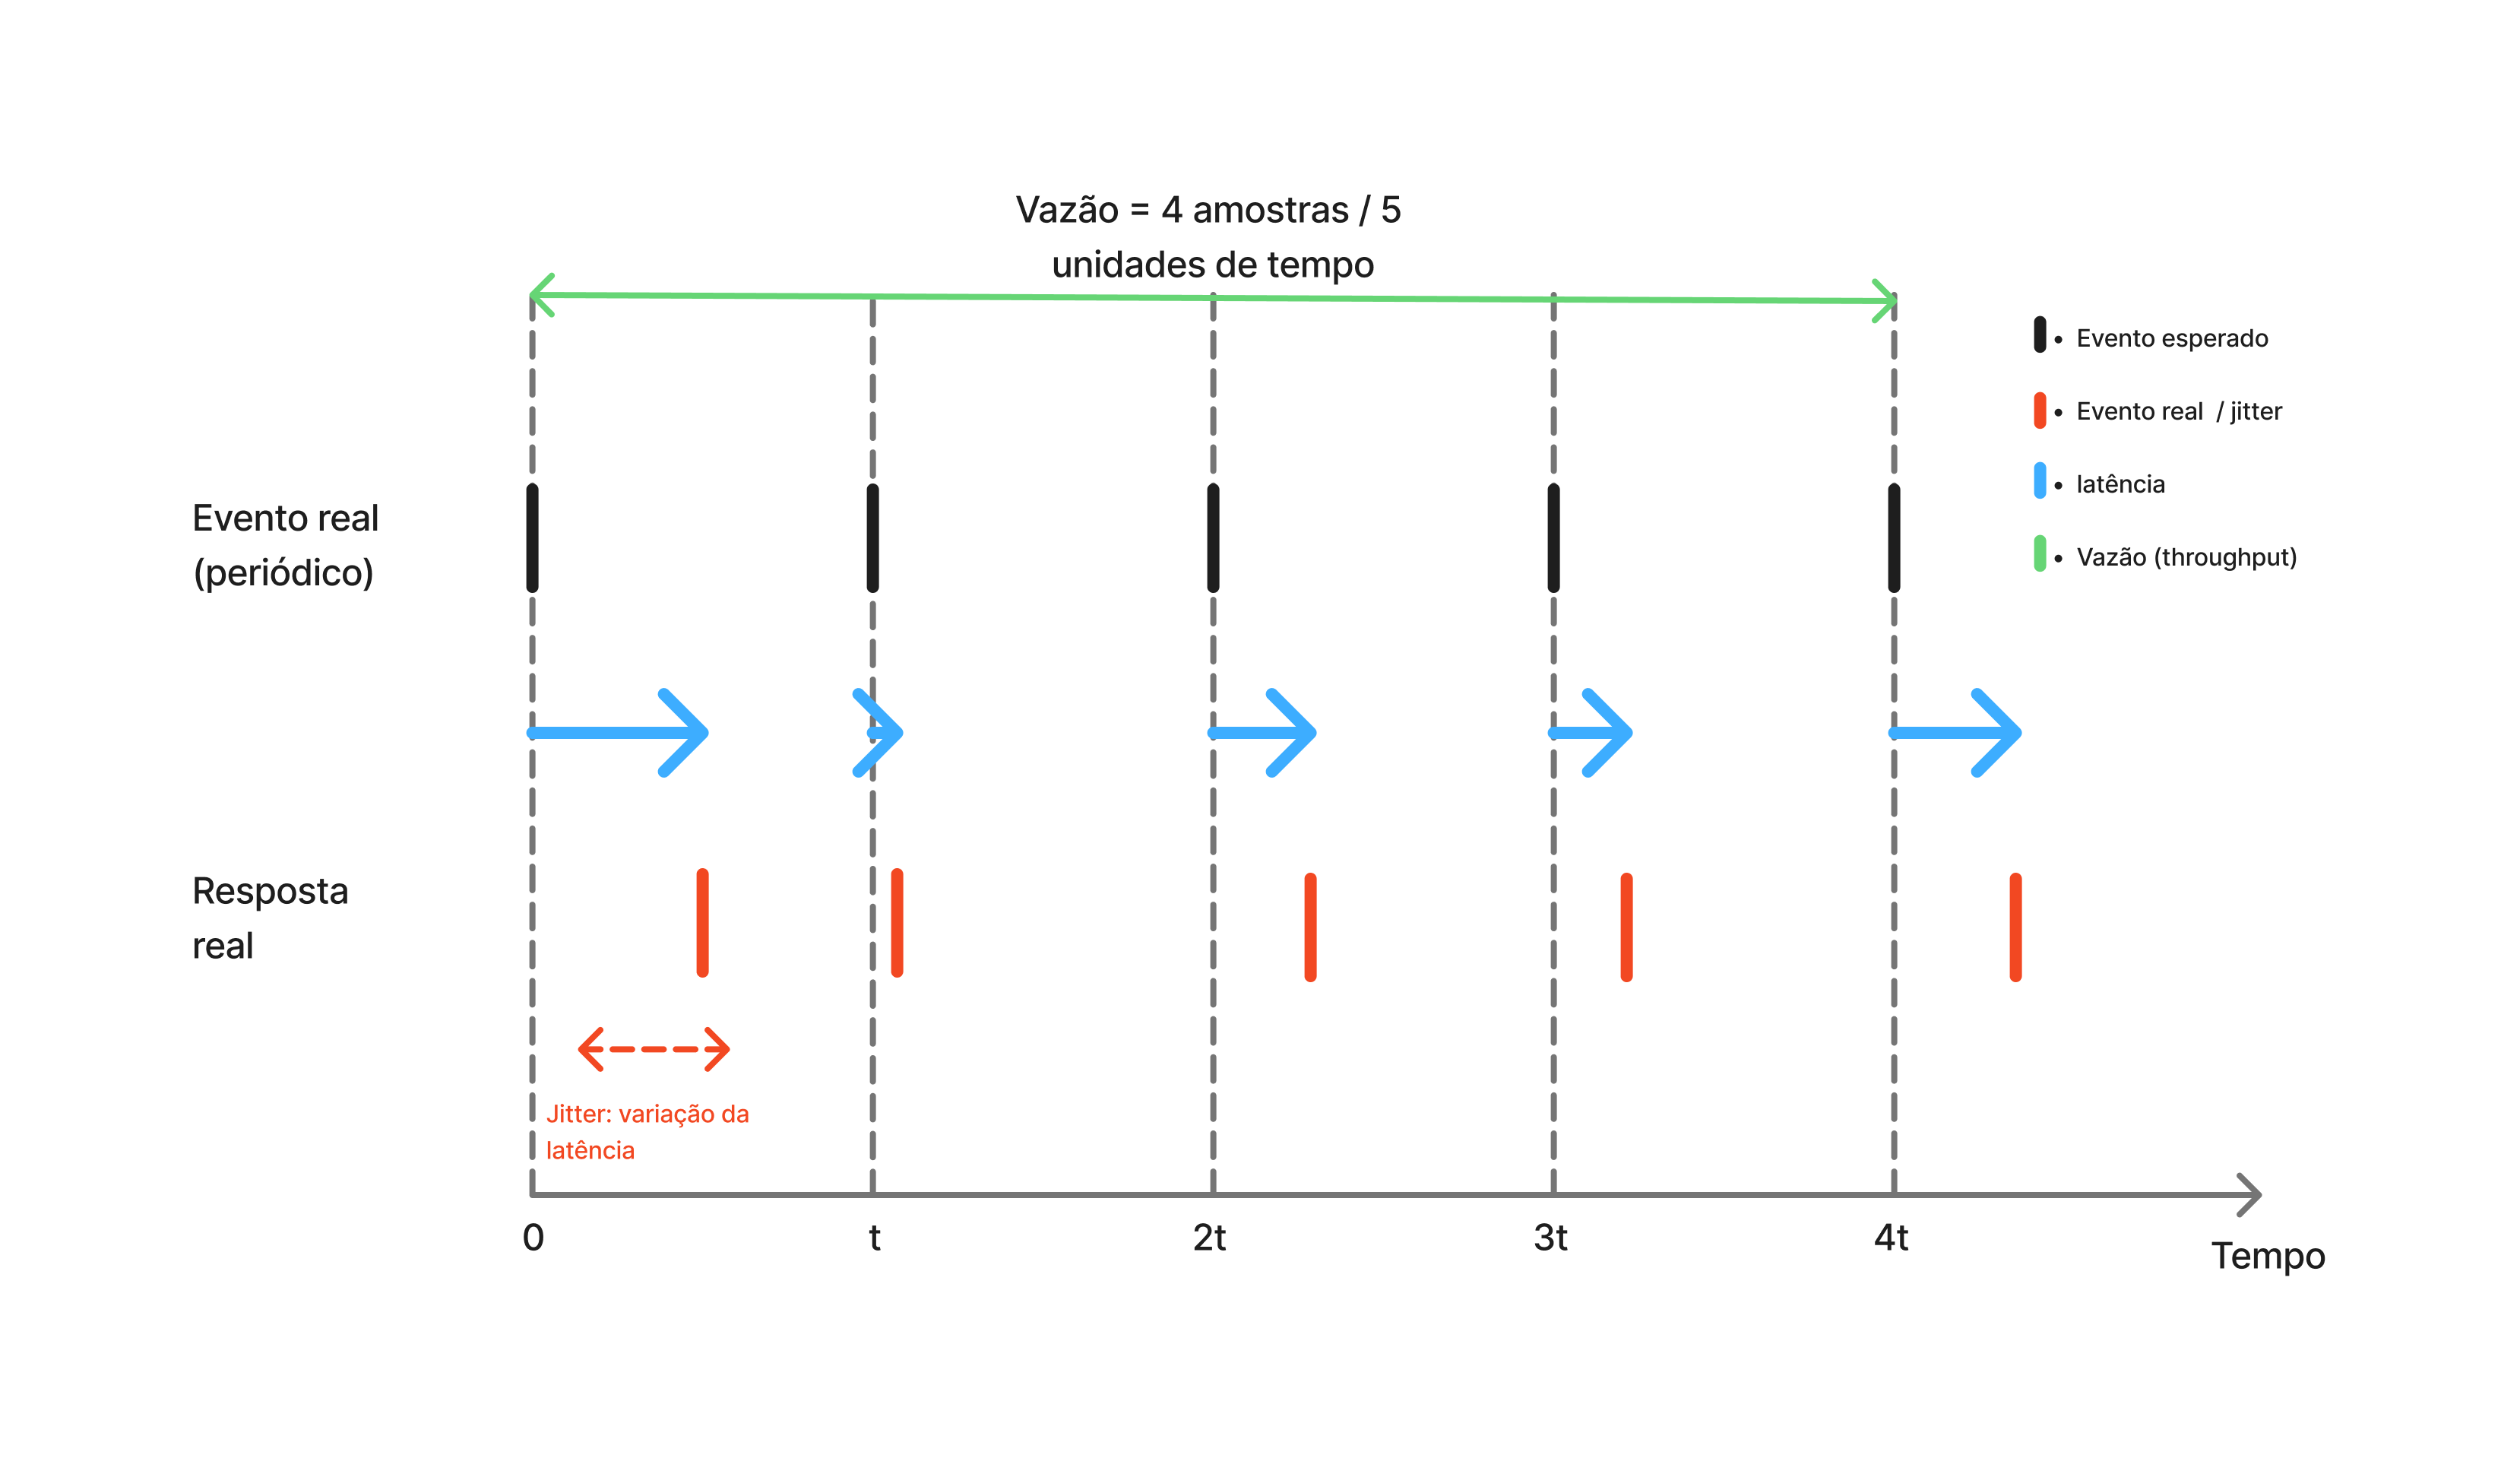
\includegraphics[width=\linewidth]{fig_2_2_latencia_jitter_vazao.png}\\[2pt]
      \src{Autoria própria.}
    \end{column}
    \begin{column}{0.46\textwidth}
      \begin{itemize}
        \setlength{\itemsep}{7pt}
        \item \textbf{Latência}: atraso entre o evento e a reação
        \item \textbf{\en{Jitter}}: variação dessa latência --- na amostragem
              periódica, variação do intervalo entre amostras
        \item \textbf{Vazão}: dados sustentados por unidade de tempo
              \emph{sem perda}
      \end{itemize}
      \vspace{4pt}
      \notebox{As quatro métricas do trabalho medem exatamente essas três
      grandezas no contexto de um instrumento.}
    \end{column}
  \end{columns}
\end{frame}

\begin{frame}{GPIO+CPU: o teto teórico é alto, mas nada protege o laço}
  \begin{columns}[T]
    \begin{column}{0.46\textwidth}
      \[ f_{s,\max} = \frac{f_{clk}}{C_{iter}} \]
      \begin{itemize}
        \setlength{\itemsep}{4pt}
        \item laço mínimo: 4 a 8 ciclos $\Rightarrow$ dezenas de MS/s
              \textbf{no melhor caso}
        \item taxa programável exige esperar um prazo a cada amostra
      \end{itemize}
      \vspace{4pt}
      \goodbox{\small No RP2350, o SIO lê \emph{todos} os pinos em uma
      instrução --- a leitura não é o gargalo.}
    \end{column}
    \begin{column}{0.50\textwidth}
      \textbf{O que alonga uma iteração}
      \begin{enumerate}
        \setlength{\itemsep}{2pt}
        \item interrupções no meio do laço (a pilha USB, entre elas)
        \item falha de cache na execução pela flash (XIP)
        \item arbitragem de barramento com DMA e periféricos
        \item o envio do bloco anterior pelo USB
      \end{enumerate}
      \alertbox{\small Interrupção como fonte de amostras é pior:
      satura em \en{livelock} e a vazão útil cai a zero.}
    \end{column}
  \end{columns}
\end{frame}

\begin{frame}{PIO+DMA: a amostra sai do caminho da CPU}
  \begin{columns}[T]
    \begin{column}{0.30\textwidth}
      \centering
      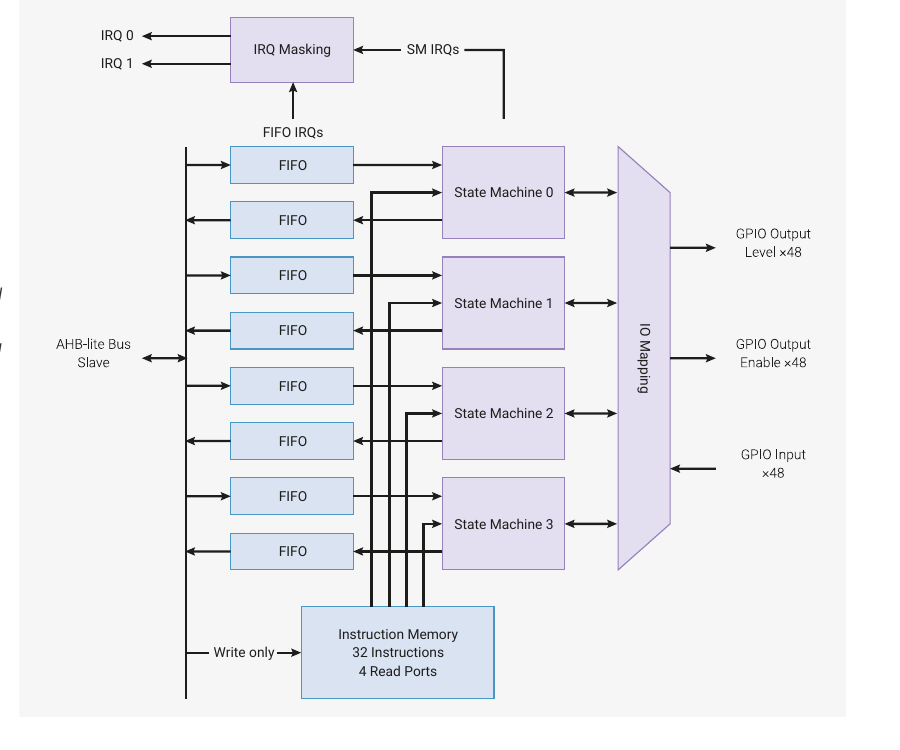
\includegraphics[width=\linewidth]{fig_2_5_pio_blocos.png}\\[2pt]
      \src{Raspberry Pi Ltd., 2024.}
    \end{column}
    \begin{column}{0.66\textwidth}
      \begin{itemize}
        \setlength{\itemsep}{4pt}
        \item \textbf{PIO}: máquinas de estado com 9 instruções de
              \textbf{1 ciclo}; taxa por divisor fracionário
              $\text{clkdiv}=f_{sys}/f_{s}$, exata em ciclos
        \item \texttt{jmp pin}: disparo por borda em \emph{hardware}
        \item \textbf{DMA} ritmada por DREQ, em \en{ping-pong}: enche um
              \en{buffer} enquanto a CPU esvazia o outro
      \end{itemize}
      \vspace{2pt}
      \goodbox{A amostra já foi tomada no instante certo: um atraso da CPU
      não vira \en{jitter}.}
      \alertbox{Em compensação, se a CPU não esvaziar a fila a tempo, há
      \en{overflow} --- perda, não deslocamento.}
    \end{column}
  \end{columns}
\end{frame}

% ===================================================================== %
\section{Como medi}
% ===================================================================== %

\begin{frame}{Dois \en{firmwares}, um só código-base}
  \begin{columns}[T]
    \begin{column}{0.49\textwidth}
      \centering\textcolor{fwA}{\textbf{Firmware A --- PIO+DMA}}\\[3pt]
      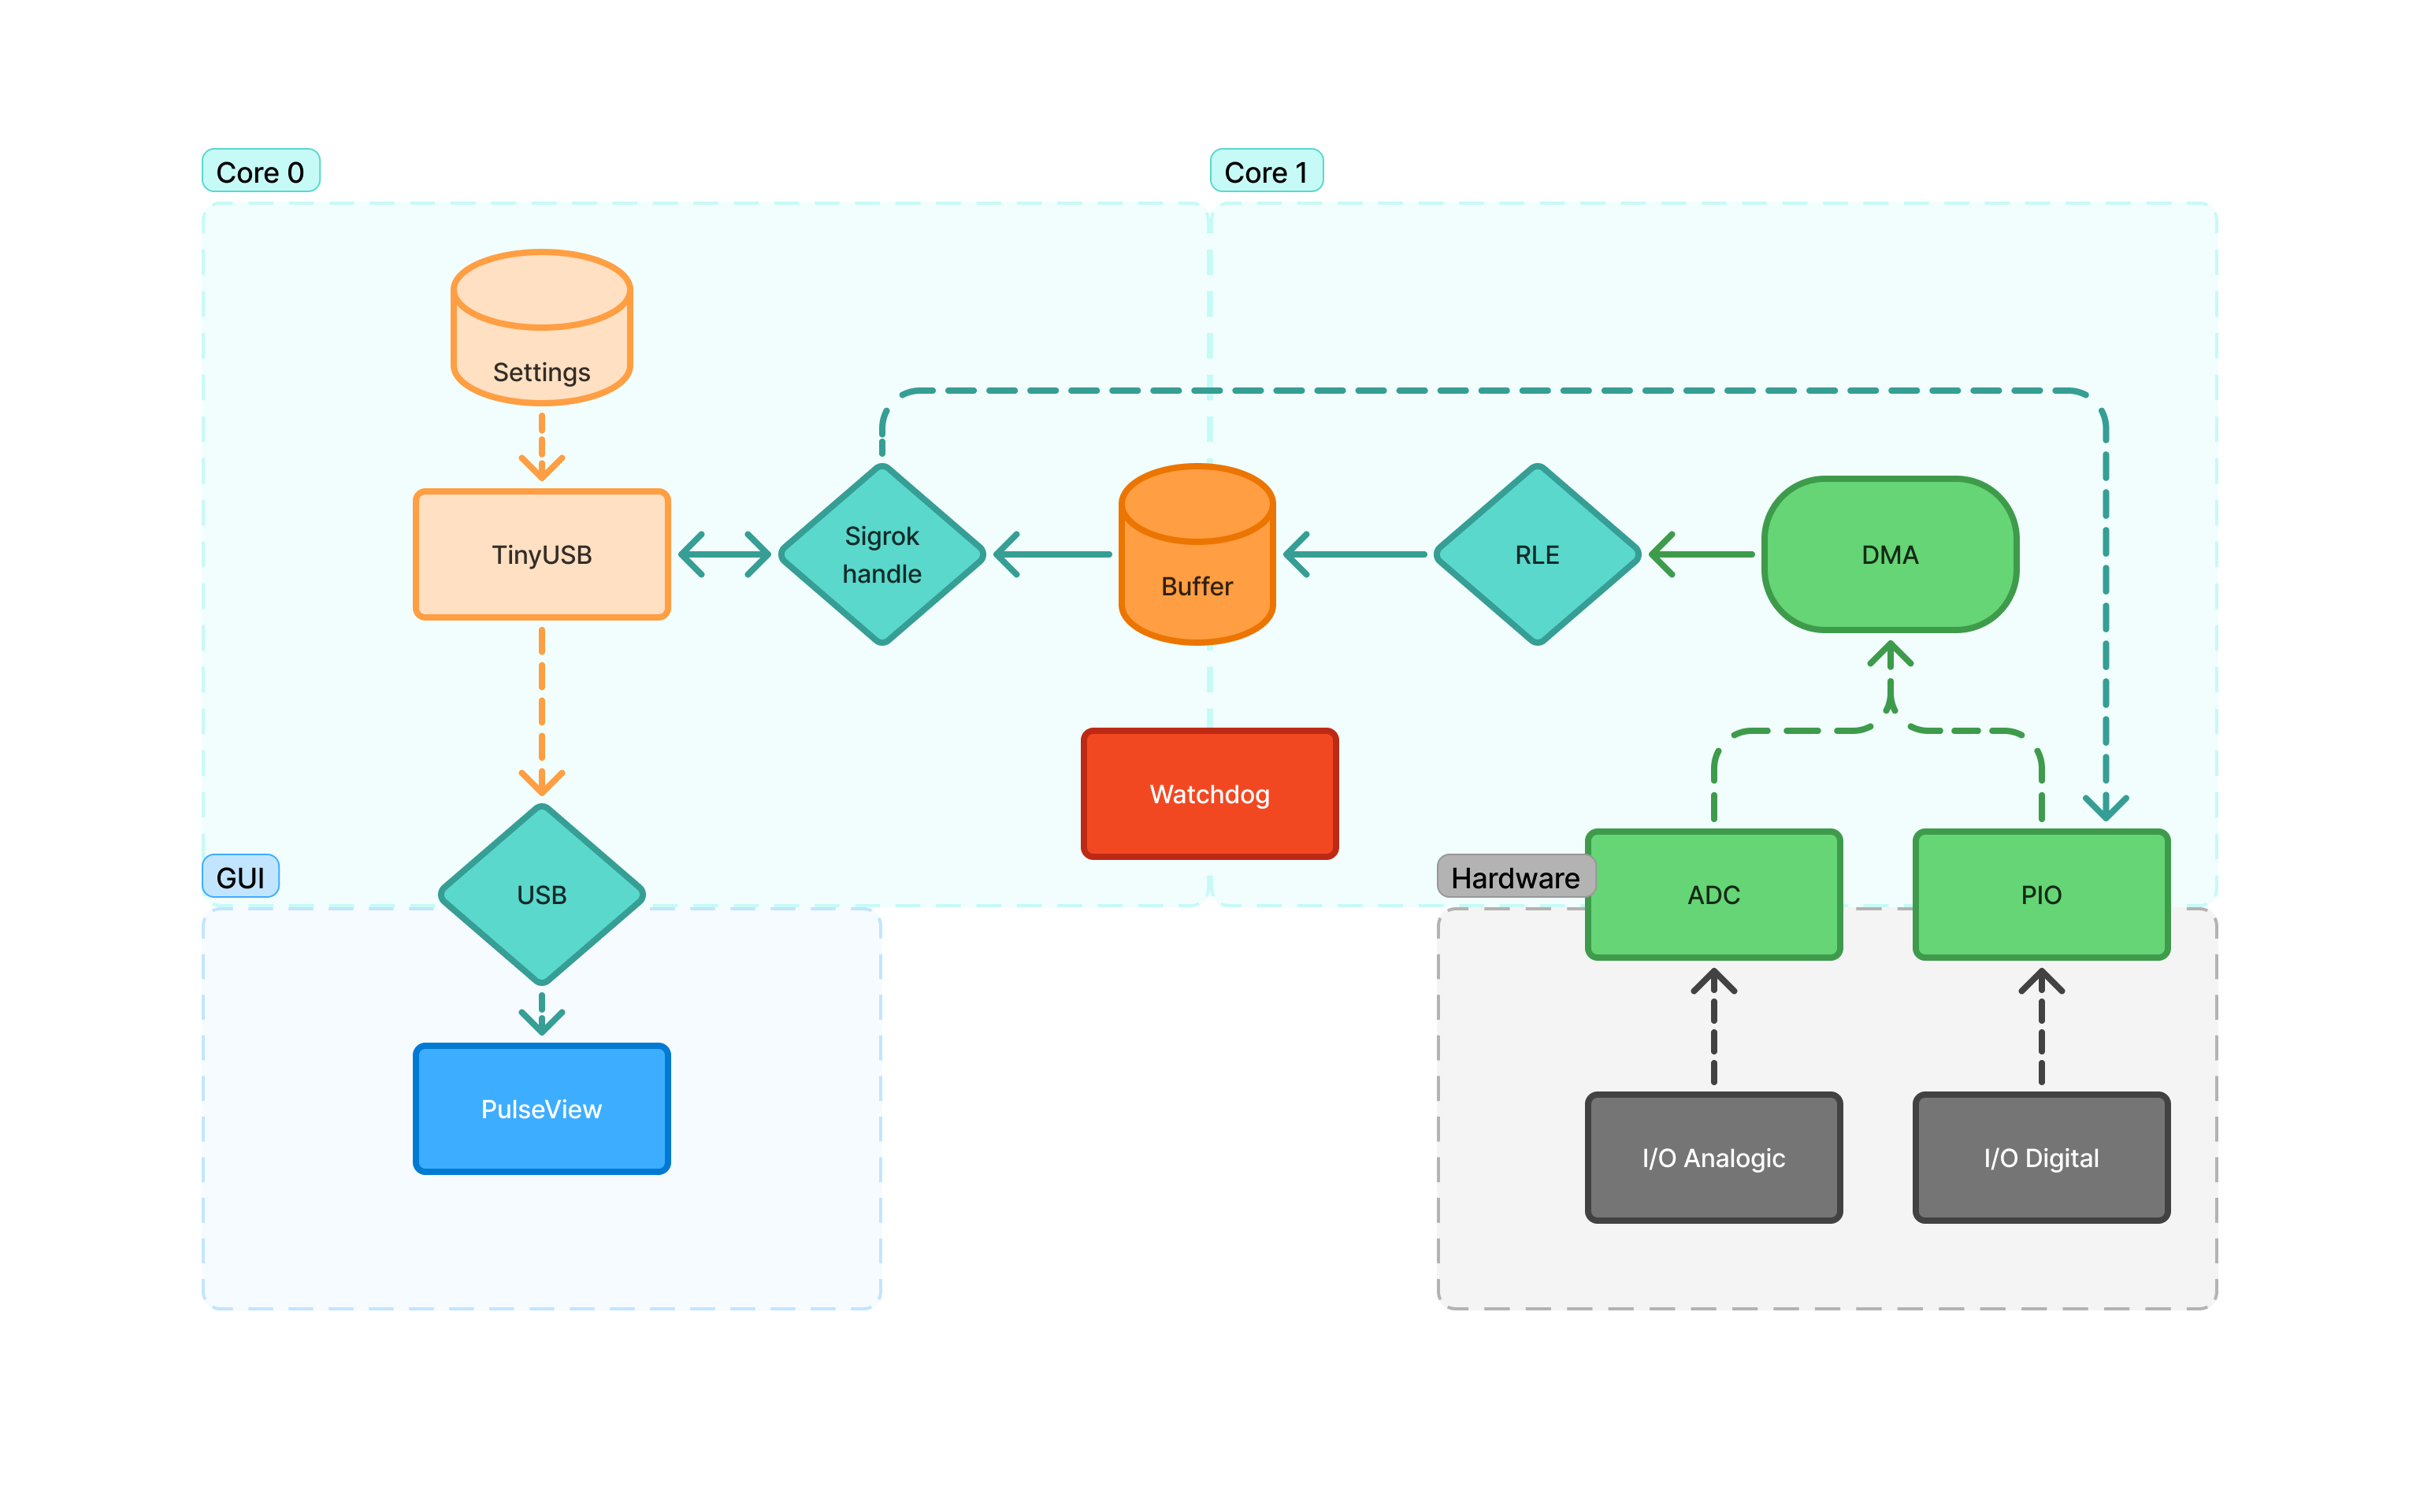
\includegraphics[height=0.39\textheight,trim=115 120 110 85,clip]{fig_3_5_arquitetura_fw_a.png}
      \begin{itemize}\small
        \item PIO amostra, DMA encadeada (2 $\times$ \num{1024} amostras)
        \item CPU só aplica RLE e envia
        \item fila estourou $\Rightarrow$ \textbf{aborta com \texttt{!!!}}
      \end{itemize}
    \end{column}
    \begin{column}{0.49\textwidth}
      \centering\textcolor{fwB}{\textbf{Firmware B --- GPIO+CPU}}\\[3pt]
      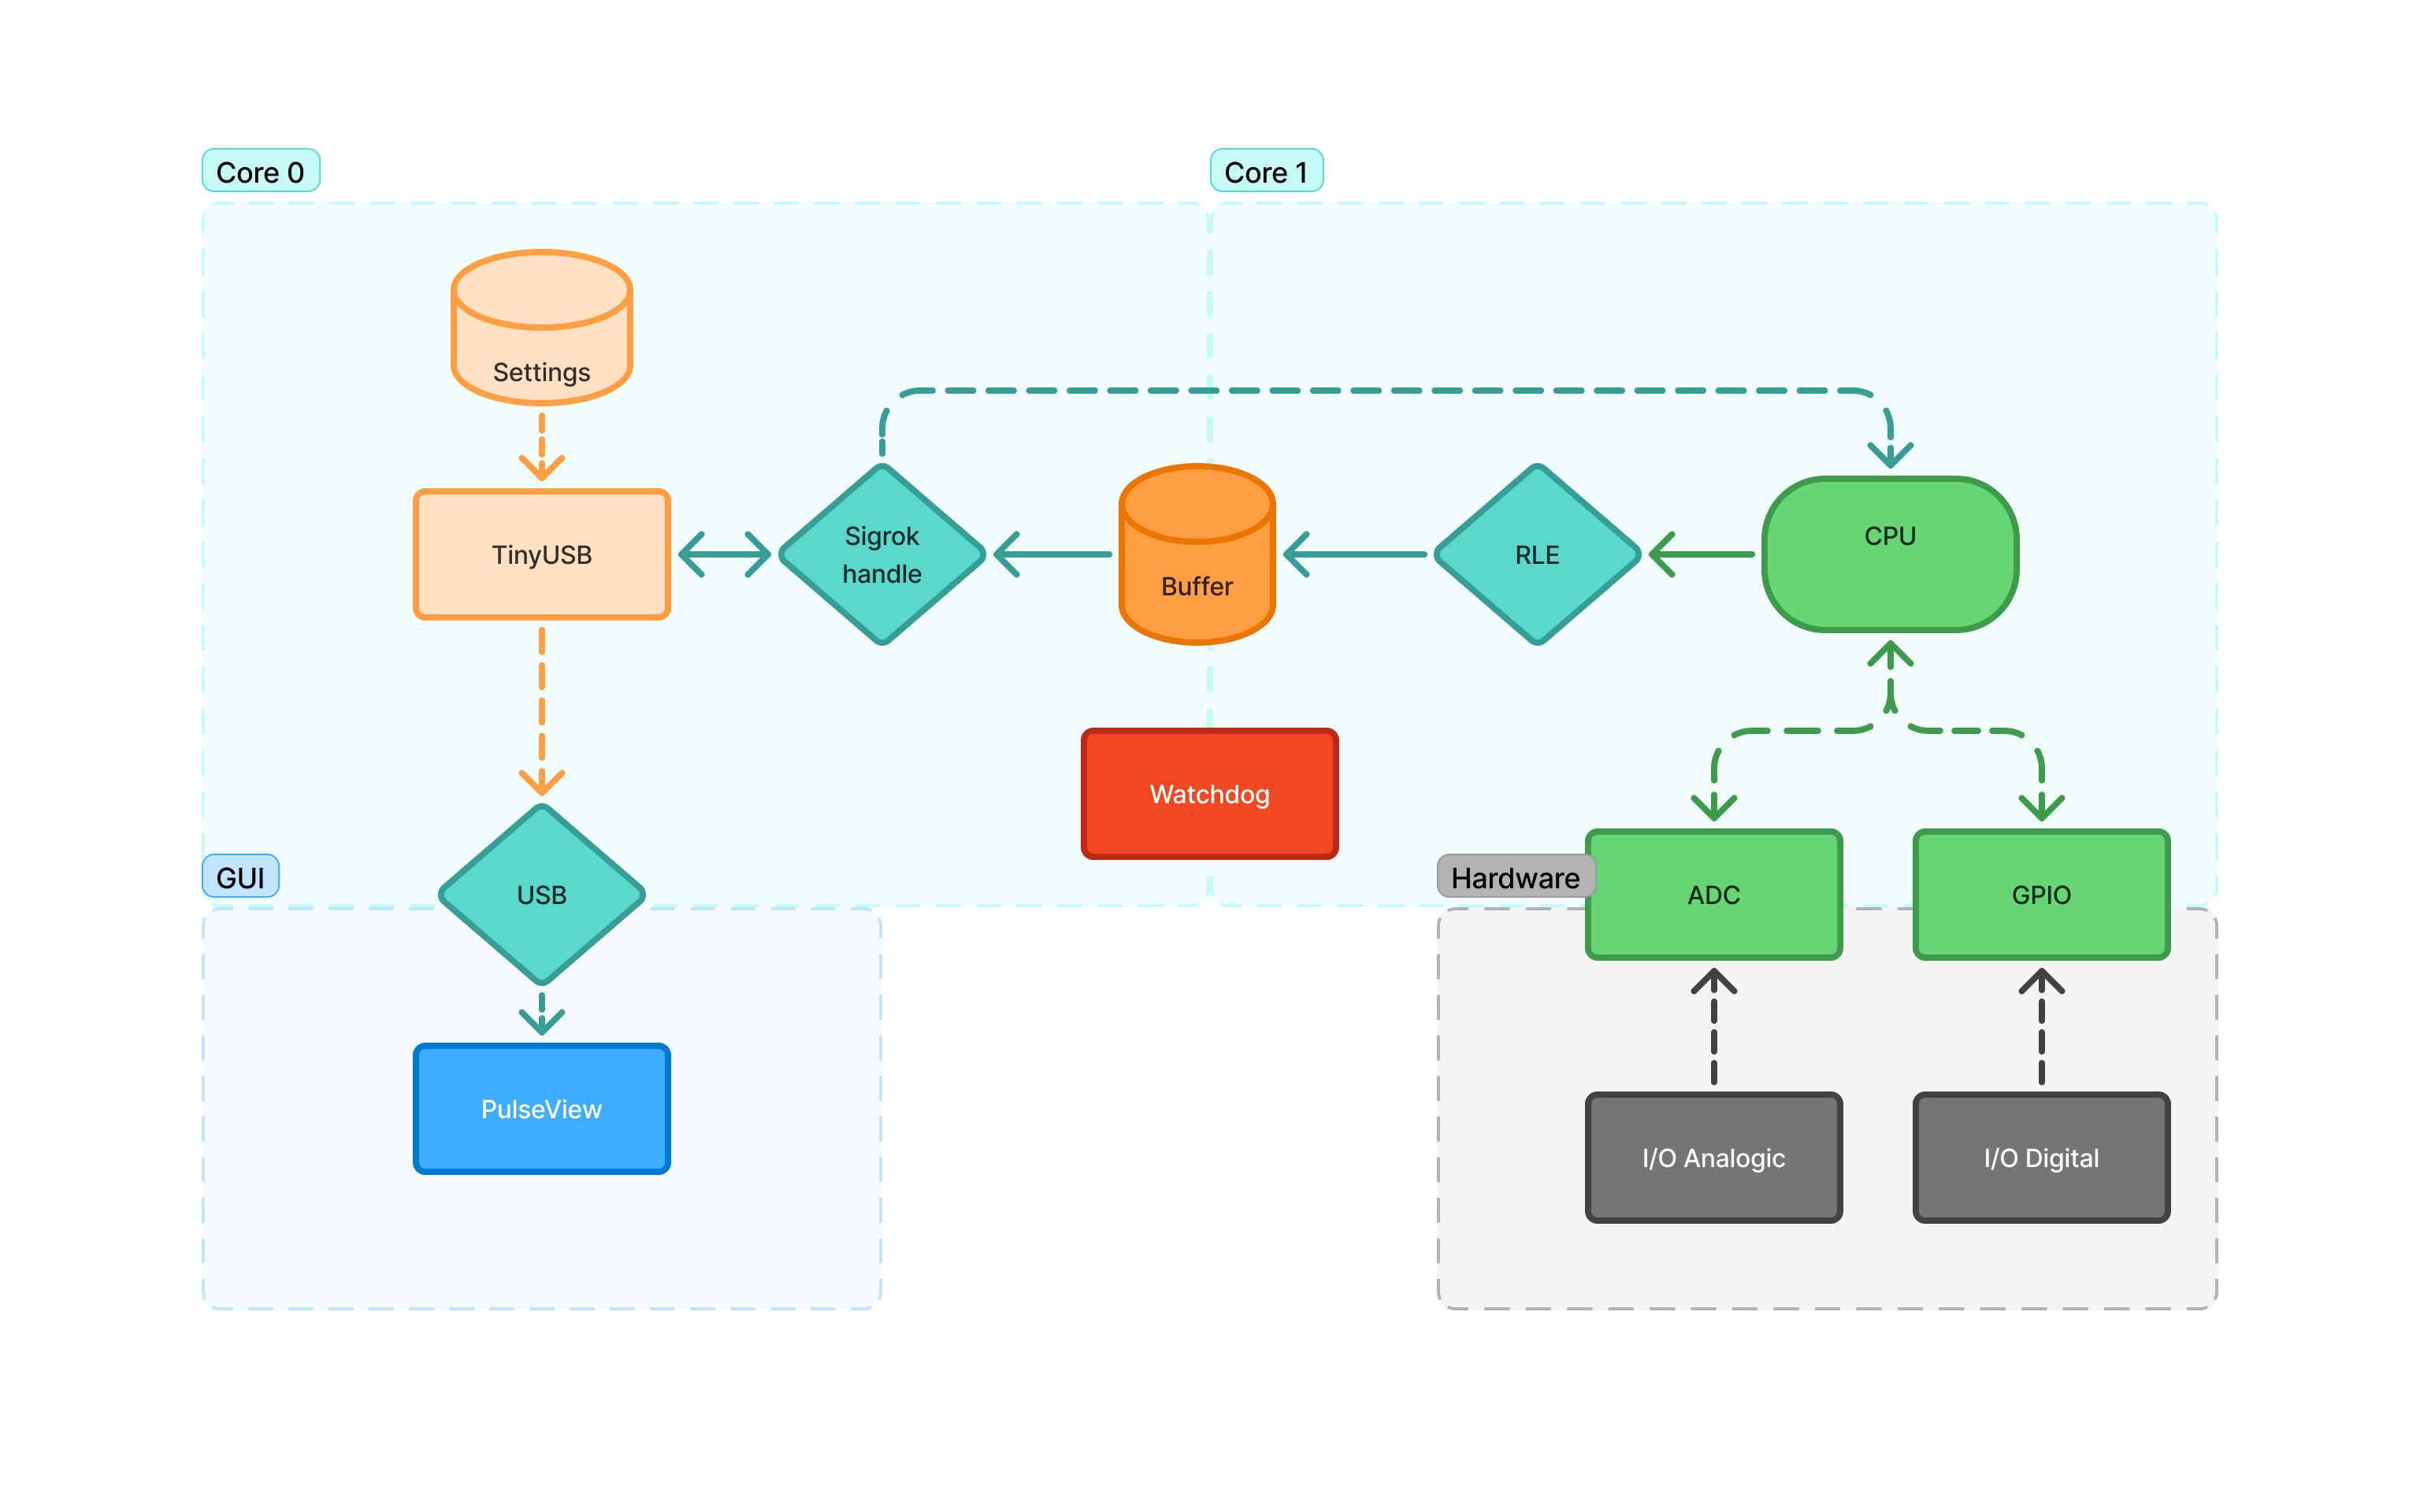
\includegraphics[height=0.39\textheight,trim=115 120 110 85,clip]{fig_3_6_arquitetura_fw_b.png}
      \begin{itemize}\small
        \item laço em C lê o SIO, prazos absolutos no contador DWT
        \item recusa taxas acima de $f_{clk}/C_{iter}$ + 5\,\%
        \item \textbf{não amostra} enquanto codifica e envia
      \end{itemize}
    \end{column}
  \end{columns}
  \vspace{2pt}
  \centering\src{Autoria própria.}
\end{frame}

\begin{frame}{A comparação só vale se uma variável mudar}
  \begin{columns}[T]
    \begin{column}{0.52\textwidth}
      \textbf{Idêntico nos dois}
      \begin{itemize}
        \setlength{\itemsep}{2pt}
        \item mesmo \en{commit} base, mesma placa, \SI{150}{MHz}
        \item protocolo sigrok-pico, RLE, TinyUSB
        \item formato das amostras e comandos
      \end{itemize}
      \vspace{7pt}
      \textbf{Diferente --- porque decorre da arquitetura}
      \begin{itemize}
        \setlength{\itemsep}{2pt}
        \item disparo: PIO $\times$ comparação em software
        \item \en{buffers}: \num{1024} em \A{} $\times$ \num{8192} em \B
      \end{itemize}
      \notebox{\small \en{Buffers} maiores $\Rightarrow$ menos pausas em B:
      a diferença \textbf{favorece B} --- que ainda assim fica atrás nas
      quatro métricas.}
    \end{column}
    \begin{column}{0.42\textwidth}
      \centering\textbf{Custo de memória}\\[4pt]
      \begin{tabular}{@{}lrr@{}}
        \toprule
        & \A & \B \\
        \midrule
        Flash      & \SI{51.7}{KB}  & \SI{46.2}{KB} \\
        BSS (SRAM) & \SI{109.2}{KB} & \SI{225.3}{KB} \\
        \% da SRAM & \SI{21.3}{\%}  & \SI{44.0}{\%} \\
        \bottomrule
      \end{tabular}\\[6pt]
      \raggedright\footnotesize\color{ufalSlate}
      B gasta o dobro da SRAM: \en{buffers} 8$\times$ maiores (+\SI{84}{KB}) e
      histórico de pré-disparo (+\SI{32}{KB}).
    \end{column}
  \end{columns}
\end{frame}

\begin{frame}{A bancada: um sinal conhecido e uma testemunha externa}
  \centering
  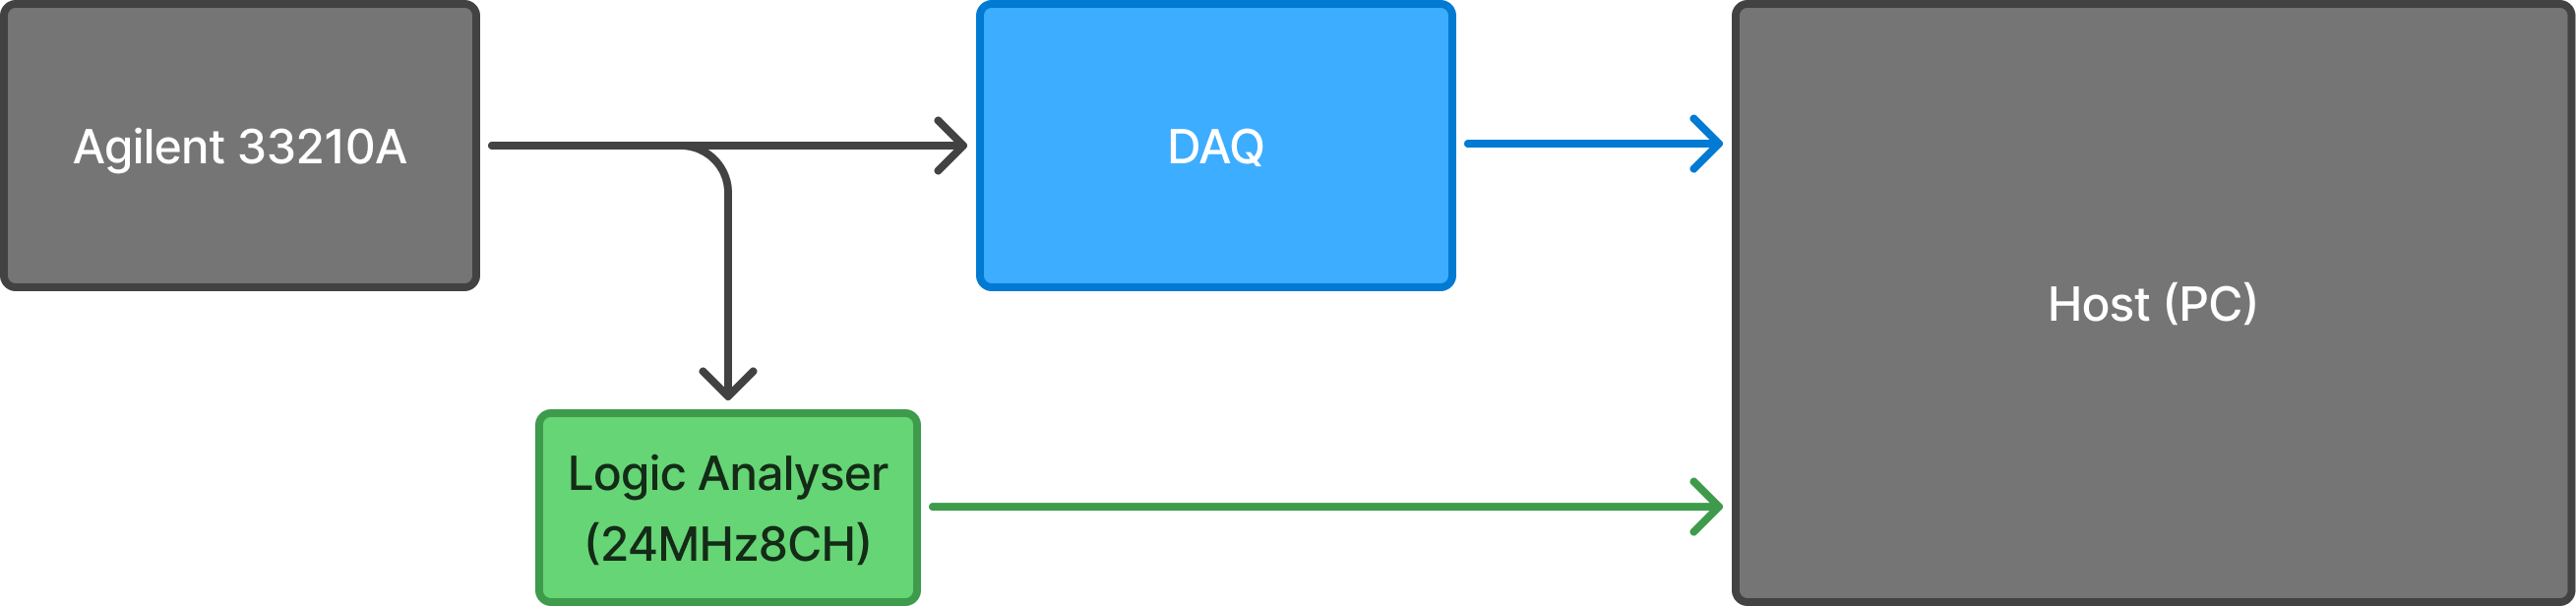
\includegraphics[width=0.80\linewidth]{fig_3_1a_bancada_diagrama.png}\\[2pt]
  \src{Autoria própria.}
  \vspace{2pt}
  \begin{columns}[T]
    \begin{column}{0.47\textwidth}
      \begin{itemize}\small
        \item gerador Agilent 33210A: onda quadrada de \SI{100}{kHz} no canal D3
        \item referência Saleae (Logic 2), armada na \emph{mesma borda} que o DAQ
      \end{itemize}
    \end{column}
    \begin{column}{0.47\textwidth}
      \begin{itemize}\small
        \item 4 e 12 canais (1 e 2 \en{bytes} por amostra)
        \item \textbf{30 repetições} por condição, \en{scripts} versionados
      \end{itemize}
    \end{column}
  \end{columns}
  \vspace{2pt}
  \punch{\normalsize O DAQ nunca é juiz de si mesmo: todo número é confrontado
  com a referência.}
\end{frame}

\begin{frame}{Quatro métricas, uma pergunta cada}
  \small
  \begin{tabularx}{\linewidth}{@{}l>{\raggedright\arraybackslash}p{3.5cm}>{\raggedright\arraybackslash}X@{}}
    \toprule
    & \textbf{Métrica} & \textbf{Pergunta que responde} \\
    \midrule
    M1 & Taxa máxima sustentada &
      Até que taxa a contagem de bordas bate com a referência? \\
    M2 & \en{Jitter} de amostragem &
      O intervalo entre amostras é constante, ou só parece? \\
    M3 & Perda em captura contínua &
      Em \SI{60}{s} de fluxo, quantas amostras chegam de fato? \\
    M4 & Ocupação de CPU &
      Quanto do processador sobra para outra tarefa? \\
    \bottomrule
  \end{tabularx}
  \vspace{8pt}
  \begin{block}{Procedimento estatístico fixado antes de medir}
    Mann--Whitney U ($\alpha = 0{,}05$) \;·\; tamanho de efeito
    \en{rank-biserial} $r$ \;·\; correção de Holm--Bonferroni por métrica
    \;·\; IC 95\,\% da diferença de medianas por \en{bootstrap}
    (\num{10000} reamostragens)
  \end{block}
\end{frame}

\begin{frame}{O critério de ``captura íntegra''}
  \begin{columns}[T]
    \begin{column}{0.54\textwidth}
      \begin{itemize}
        \setlength{\itemsep}{6pt}
        \item Janela de \SI{0.2}{s} a \SI{100}{kHz}: a referência registra
              exatamente \textbf{\num{20000} bordas de subida}
        \item Íntegra = contagem do DAQ bate com a da referência dentro de
              \textbf{0,1\,\%} (\num{20} bordas)
        \item Critério estrito de sensibilidade: \textbf{$\pm$2 bordas},
              o suficiente para absorver o corte da janela
      \end{itemize}
    \end{column}
    \begin{column}{0.42\textwidth}
      \notebox{Contar bordas \emph{a mais} é impossível se o fluxo for
      contínuo: indica que a captura cobriu mais tempo do que diz cobrir.}
      \vspace{6pt}
      \alertbox{É esse detalhe que vai separar os dois \en{firmwares}.}
    \end{column}
  \end{columns}
\end{frame}

% ===================================================================== %
\section{Resultados}
% ===================================================================== %

\begin{frame}{M1: A sustenta \SI{3.66}{MS/s}; B, entre \SI{2.48}{MS/s} e \SI{774.6}{kS/s}}
  \begin{columns}[T]
    \begin{column}{0.62\textwidth}
      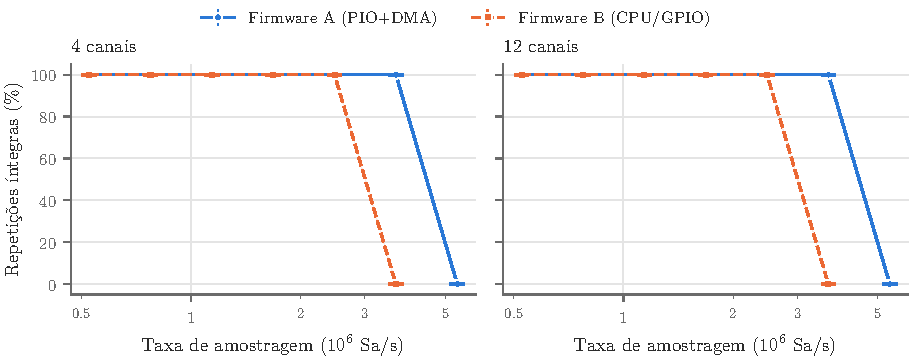
\includegraphics[width=\linewidth]{fig_4_1_m1_integras.pdf}\\[2pt]
      \src{Autoria própria.}
    \end{column}
    \begin{column}{0.35\textwidth}
      \begin{itemize}
        \setlength{\itemsep}{6pt}
        \item \A: contagem exata em 30/30 repetições até \SI{3.66}{MS/s};
              acima, \emph{aborta e sinaliza}
        \item \B: \SI{2.48}{MS/s} pelo critério de 0,1\,\%;
              \SI{774.6}{kS/s} pelo de $\pm$2 bordas
      \end{itemize}
      \vspace{4pt}
      \bignumber{1,5--4,7$\times$}{taxa de A em relação à de B}
    \end{column}
  \end{columns}
\end{frame}

\begin{frame}{M1: B entrega bordas \emph{a mais} --- e não avisa}
  \begin{columns}[T]
    \begin{column}{0.60\textwidth}
      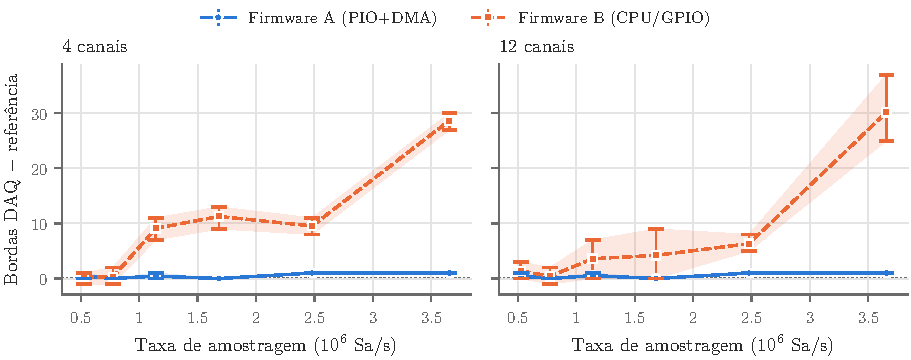
\includegraphics[width=\linewidth]{fig_4_2_m1_excesso_bordas.pdf}\\[2pt]
      \src{Autoria própria.}
    \end{column}
    \begin{column}{0.37\textwidth}
      \begin{itemize}
        \setlength{\itemsep}{4pt}
        \item O laço de B \emph{pausa} para transmitir e retoma sem marcar
        \item O \en{host} supõe amostras igualmente espaçadas: a janela
              ``de \SI{0.2}{s}'' cobre mais tempo real
        \item Separação completa desde \SI{1.14}{MS/s} ($r \ge +0{,}90$)
      \end{itemize}
      \alertbox{\small Não é falta de ciclos: $C_{iter}=35$ dá teto de
      \SI{4.29}{MS/s}, e B falha em 85\,\% dele.}
    \end{column}
  \end{columns}
\end{frame}

\begin{frame}{M2: o \en{jitter} de A é só quantização; o de B, centenas de ns}
  \begin{columns}[T]
    \begin{column}{0.60\textwidth}
      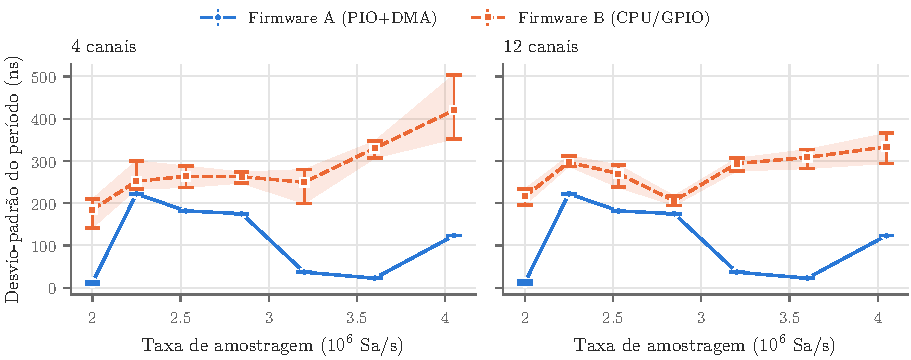
\includegraphics[width=\linewidth]{fig_4_3_m2_jitter_std.pdf}\\[2pt]
      \src{Autoria própria.}
    \end{column}
    \begin{column}{0.37\textwidth}
      \[ \sigma_q = T_s\sqrt{\varphi(1-\varphi)} \]
      \begin{itemize}
        \setlength{\itemsep}{4pt}
        \item \A: $\sigma$ igual ao limite de quantização
              (diferença $\le$ \SI{3.6}{ns}), repetível entre capturas
        \item \B: \textbf{106 a \SI{400}{ns}} acima de $\sigma_q$ ---
              16 a 60 ciclos de CPU
      \end{itemize}
      \goodbox{\small Separação completa nas 14 condições: $r = +1{,}00$.}
    \end{column}
  \end{columns}
\end{frame}

\begin{frame}{M2: em B, uma pausa chega a engolir um pulso inteiro}
  \begin{columns}[T]
    \begin{column}{0.56\textwidth}
      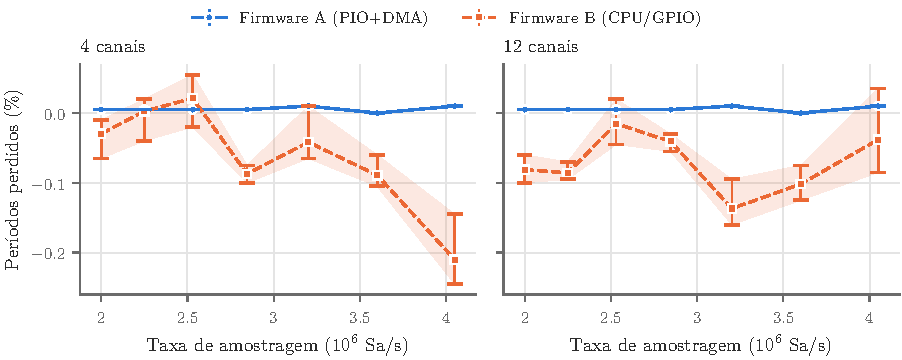
\includegraphics[width=\linewidth]{fig_4_4_m2_periodos_perdidos.pdf}\\[2pt]
      \src{Autoria própria.}
    \end{column}
    \begin{column}{0.41\textwidth}
      \begin{itemize}
        \setlength{\itemsep}{5pt}
        \item Valor pico a pico do período: 0,25 a \SI{1.0}{\micro s} em \A{}
              contra 6,3 a \SI{13.3}{\micro s} em \B
        \item \SI{13}{\micro s} $\approx$ dois períodos do sinal: duas bordas
              viraram uma
        \item A contagem de períodos repete o padrão da M1: até \textbf{42 a
              mais} em \SI{4.05}{MS/s}
      \end{itemize}
      \notebox{\small O \en{jitter} ciclo a ciclo não explica isso --- é o
      mesmo mecanismo de pausa.}
    \end{column}
  \end{columns}
\end{frame}

\begin{frame}{M3: em \SI{60}{s} de captura, B deixa de amostrar 14 a \SI{26}{s}}
  \begin{columns}[T]
    \begin{column}{0.58\textwidth}
      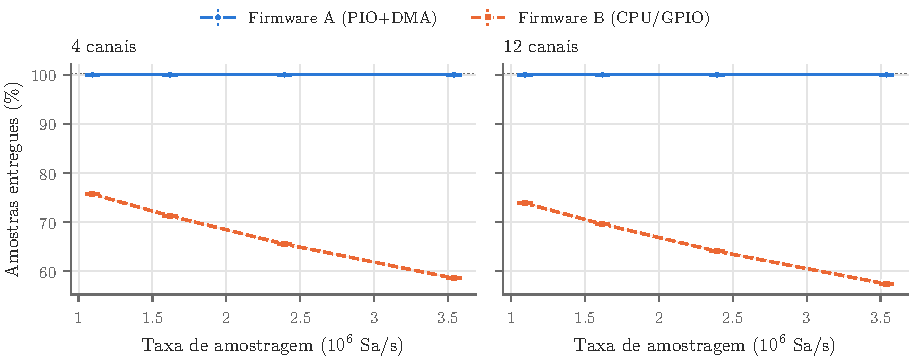
\includegraphics[width=\linewidth]{fig_4_5_m3_entregues.pdf}\\[2pt]
      \src{Autoria própria.}
    \end{column}
    \begin{column}{0.39\textwidth}
      \begin{itemize}
        \setlength{\itemsep}{4pt}
        \item \A: \textbf{100\,\%} das amostras e \textbf{zero} lacunas até
              \SI{3.54}{MS/s}; em \SI{5.24}{MS/s}, aborta
        \item \B: \textbf{57 a 76\,\%} entregues já a partir de
              \SI{1.09}{MS/s}, \emph{sem nenhuma marca no fluxo}
        \item Variação $<$ 0,1 p.p.\ entre repetições: perda
              \textbf{sistemática}
      \end{itemize}
      \bignumber{14--26\,s}{sem amostrar, a cada \SI{60}{s}, em B}
    \end{column}
  \end{columns}
\end{frame}

\begin{frame}{M3: a perda não vem do USB --- vem de dividir a CPU}
  \begin{columns}[T]
    \begin{column}{0.58\textwidth}
      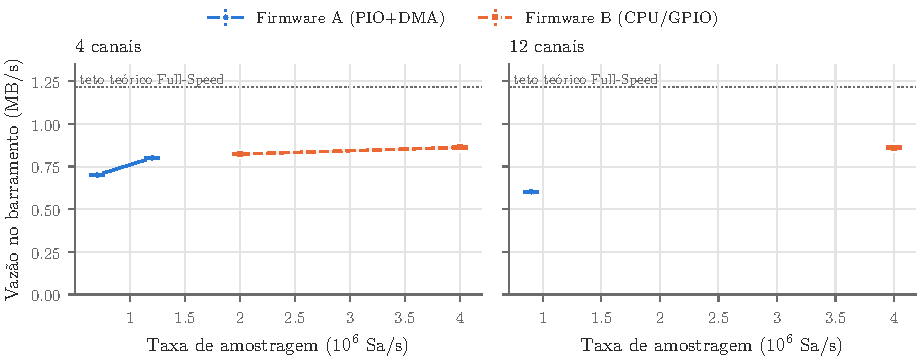
\includegraphics[width=\linewidth]{fig_4_8_usb_vazao.pdf}\\[2pt]
      \src{Autoria própria.}
    \end{column}
    \begin{column}{0.39\textwidth}
      \begin{itemize}
        \setlength{\itemsep}{5pt}
        \item Com o mesmo sinal e o mesmo barramento, \A{} entrega 100\,\%:
              logo, o USB não é o limite de B
        \item Com sinal pouco compressível, \B{} satura em
              $\approx$\SI{0.86}{MB/s} (71\,\% do Full-Speed) e entrega
              15 a 42\,\%
        \item \A{} sustenta até $\approx$\SI{0.80}{MB/s}; acima de
              $\approx$\SI{0.92}{MB/s}, \emph{aborta} em vez de descartar
      \end{itemize}
    \end{column}
  \end{columns}
\end{frame}

\begin{frame}{M4: B ocupa 100\,\% da CPU; A, proporcional à taxa}
  \begin{columns}[T]
    \begin{column}{0.60\textwidth}
      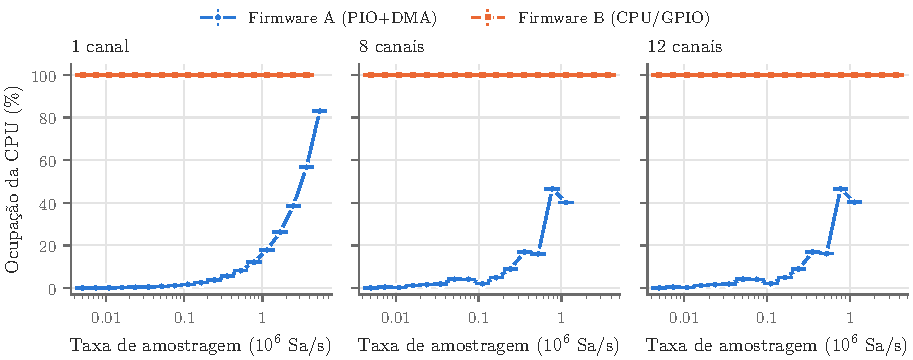
\includegraphics[width=\linewidth]{fig_4_9_m4_ocupacao.pdf}\\[2pt]
      \src{Autoria própria.}
    \end{column}
    \begin{column}{0.37\textwidth}
      \begin{itemize}
        \setlength{\itemsep}{4pt}
        \item \B: \textbf{100\,\%} em qualquer taxa, inclusive \SI{5}{kS/s}
              --- espera ativa pelo prazo da amostra
        \item \A: de \textbf{0,08\,\%} a \textbf{83\,\%}, porque a CPU ainda
              percorre cada amostra no RLE ($\approx$23 ciclos/amostra)
      \end{itemize}
      \notebox{\small PIO+DMA tira a CPU da \textbf{amostragem}, não do
      \textbf{processamento} do fluxo.}
    \end{column}
  \end{columns}
\end{frame}

\begin{frame}{Resumo: separação completa em praticamente tudo}
  \small
  \begin{tabularx}{\linewidth}{@{}l>{\raggedright\arraybackslash}X>{\raggedright\arraybackslash}X@{}}
    \toprule
    & \fwA{} (PIO+DMA) & \fwB{} (GPIO+CPU) \\
    \midrule
    M1 & \SI{3.66}{MS/s}, contagem exata; aborto sinalizado acima &
         \SI{2.48}{MS/s} (\SI{774.6}{kS/s} pelo critério estrito); bordas a mais \\
    M2 & $\sigma$ = limite de quantização, repetível &
         +106 a \SI{400}{ns}; pico a pico até \SI{13}{\micro s} \\
    M3 & 100\,\% das amostras, zero lacunas até \SI{3.54}{MS/s} &
         57 a 76\,\%, sem sinalização, desde \SI{1.09}{MS/s} \\
    M4 & 0,08 a 83\,\% (custo do RLE) & 100\,\% em qualquer taxa \\
    \bottomrule
  \end{tabularx}
  \vspace{8pt}
  \notebox{Na maioria das condições o efeito é o máximo possível
  ($|r| = 1$): \emph{todas} as repetições de um \en{firmware} ficam de um lado
  de \emph{todas} as do outro.}
\end{frame}

% ===================================================================== %
\section{O que isso significa}
% ===================================================================== %

\begin{frame}{A diferença decisiva não é a taxa: é o modo de falhar}
  \begin{columns}[T]
    \begin{column}{0.48\textwidth}
      \begin{exampleblock}{\fwA{}: falha explícita}
        Dentro da faixa, fluxo exato e repetível.\\[3pt]
        Fora dela, \textbf{aborta} com \texttt{!!!}: o usuário sabe que a
        captura não vale.
      \end{exampleblock}
    \end{column}
    \begin{column}{0.48\textwidth}
      \begin{alertblock}{\fwB{}: falha silenciosa}
        O laço para enquanto transmite e o fluxo não marca as pausas.\\[3pt]
        A captura \textbf{parece válida}, mas a escala de tempo não é a real.
      \end{alertblock}
    \end{column}
  \end{columns}
  \vspace{8pt}
  \punch{Para um instrumento de medição, degradar em silêncio\\
  é mais grave do que recusar a captura.}
  \centering{\small\color{ufalSlate}O usuário não distingue isso de um
  comportamento real do circuito medido.}
\end{frame}

\begin{frame}{Quando cada arquitetura basta}
  \begin{columns}[T]
    \begin{column}{0.48\textwidth}
      \textcolor{fwB}{\textbf{GPIO+CPU basta}}
      \begin{itemize}
        \setlength{\itemsep}{4pt}
        \item capturas curtas, com disparo e janela fixa
        \item até $\approx$\SI{774.6}{kS/s}, com contagem exata
        \item quando centenas de ns de incerteza por amostra são aceitáveis
      \end{itemize}
    \end{column}
    \begin{column}{0.48\textwidth}
      \textcolor{fwA}{\textbf{PIO+DMA é indispensável}}
      \begin{itemize}
        \setlength{\itemsep}{4pt}
        \item acima de $\approx$\SI{1.1}{MS/s} com disparo
        \item em captura contínua, já desde \SI{1.09}{MS/s}
        \item quando a integridade do fluxo importa
        \item quando a CPU precisa ficar livre
      \end{itemize}
    \end{column}
  \end{columns}
  \vspace{10pt}
  \punch{\normalsize A escolha passa a ser uma decisão medida, e não uma
  intuição sobre o periférico disponível.}
\end{frame}

\begin{frame}{O teto de A também não é do PIO}
  \begin{columns}[T]
    \begin{column}{0.52\textwidth}
      \begin{itemize}
        \setlength{\itemsep}{6pt}
        \item O PIO amostra a dezenas de MS/s; o limite está em
              \textbf{consumir} as amostras
        \item Dois gargalos, ambos corrigíveis sem trocar de arquitetura:
          \begin{itemize}
            \item RLE na CPU ($\approx$23 ciclos/amostra)
            \item fila de apenas dois \en{buffers}
                  ($\approx$\SI{0.4}{ms} a \SI{5}{MS/s})
          \end{itemize}
      \end{itemize}
    \end{column}
    \begin{column}{0.44\textwidth}
      \notebox{O projeto \emph{gusmanb} atinge \SI{100}{MS/s} com o mesmo
      PIO+DMA no RP2040 --- porque grava em SRAM e só transmite \emph{depois}
      da captura.}
      \vspace{6pt}
      \goodbox{\small São dois pontos da mesma troca entre \textbf{taxa} e
      \textbf{duração}, não arquiteturas diferentes.}
    \end{column}
  \end{columns}
  \vspace{4pt}
  \punch{\normalsize Tirar a CPU da amostragem foi metade do caminho;
  a outra metade é tirá-la do fluxo.}
\end{frame}

\begin{frame}{A metodologia também produziu resultado}
  \begin{columns}[T]
    \begin{column}{0.56\textwidth}
      \begin{itemize}
        \setlength{\itemsep}{6pt}
        \item A referência externa revelou um defeito na \textbf{primeira
              versão do Firmware A}: ela rearmava PIO e DMA a cada bloco e
              deixava lacunas de $\approx$\SI{1.5}{\micro s} \emph{não
              sinalizadas}
        \item Sintoma idêntico ao de B --- bordas a mais --- e teto preso em
              \SI{774.6}{kS/s}
        \item Corrigido com DMA encadeada em \en{ping-pong} também no disparo;
              depois disso, \textbf{zero lacunas em 240 capturas} de \SI{60}{s}
      \end{itemize}
    \end{column}
    \begin{column}{0.40\textwidth}
      \alertbox{Sem a testemunha externa, essa falha teria passado por
      resultado.}
      \vspace{8pt}
      \goodbox{\small O mesmo método que comparou as arquiteturas serviu para
      validar o instrumento.}
    \end{column}
  \end{columns}
\end{frame}

% ===================================================================== %
\section{Conclusão}
% ===================================================================== %

\begin{frame}{Conclusões}
  \begin{columns}[T]
    \begin{column}{0.56\textwidth}
      \begin{itemize}
        \setlength{\itemsep}{5pt}
        \item Objetivos atendidos: segunda arquitetura no mesmo \en{firmware},
              quatro métricas instrumentadas, bancada automatizada com
              referência externa
        \item \textbf{Contribuição}: a comparação controlada que faltava, e o
              ponto em que a leitura por software deixa de ser confiável
        \item A causa da falha de B não é o custo do laço: é a CPU dividida
              entre amostrar e transmitir
        \item \en{Firmwares}, \en{scripts} e dados brutos versionados para
              reprodução
      \end{itemize}
    \end{column}
    \begin{column}{0.40\textwidth}
      \begin{columns}[T]
        \begin{column}{0.5\linewidth}
          \bignumber{4,7$\times$}{taxa sustentada\\(critério estrito)}
        \end{column}
        \begin{column}{0.5\linewidth}
          \bignumber{100\,\%}{amostras entregues\\por A em \SI{60}{s}}
        \end{column}
      \end{columns}
      \vspace{14pt}
      \begin{columns}[T]
        \begin{column}{0.5\linewidth}
          \bignumber{$\sigma_q$}{\en{jitter} de A:\\só quantização}
        \end{column}
        \begin{column}{0.5\linewidth}
          \bignumber{100\,\%}{CPU ocupada\\em B}
        \end{column}
      \end{columns}
    \end{column}
  \end{columns}
\end{frame}

\begin{frame}{Limitações e trabalhos futuros}
  \begin{columns}[T]
    \begin{column}{0.48\textwidth}
      \textbf{Limitações}
      \begin{itemize}
        \setlength{\itemsep}{3pt}
        \item um só sinal (\SI{100}{kHz}, um canal) em M1--M3
        \item só a variante de núcleo único de B
        \item \en{buffers} diferentes entre A e B (favorece B)
        \item uma placa, um \en{host}, referência sem calibração rastreável
        \item números específicos do RP2350 a \SI{150}{MHz}
      \end{itemize}
    \end{column}
    \begin{column}{0.48\textwidth}
      \textbf{Trabalhos futuros}
      \begin{itemize}
        \setlength{\itemsep}{3pt}
        \item \textbf{B com dois núcleos}: o único que pode mudar a conclusão
              prática
        \item RLE no PIO ou no segundo núcleo; fila de DMA mais profunda
        \item fontes do \en{jitter} de B: XIP $\times$ SRAM, IRQ ligadas
              $\times$ desligadas
        \item verificação externa por osciloscópio em pino de \en{debug}
        \item mais sinais e canais; latência de disparo; protocolos reais
      \end{itemize}
    \end{column}
  \end{columns}
\end{frame}

\begin{frame}{Referências principais}
  \footnotesize
  \begin{itemize}
    \setlength{\itemsep}{3pt}
    \item RASPBERRY PI LTD. \textbf{RP2350 Datasheet}. Cambridge, UK, 2024.
    \item PICO-CODER. \textbf{sigrok-pico}: logic analyzer and oscilloscope
          with sigrok. Repositório GitHub, 2023.
    \item GUSMANB. \textbf{LogicAnalyzer}: logic analyzer hardware and
          software. Repositório GitHub, s.d.
    \item MOGUL, J. C.; RAMAKRISHNAN, K. K. Eliminating receive livelock in an
          interrupt-driven kernel. \textbf{ACM Transactions on Computer
          Systems}, v. 15, n. 3, p. 217--252, ago. 1997.
    \item REGEHR, J.; DUONGSAA, U. Preventing interrupt overload. In:
          \textbf{Proceedings of the LCTES 2005}. [S.l.]: ACM, 2005. p. 50--58.
    \item KALIBERA, T.; JONES, R. Rigorous benchmarking in reasonable time. In:
          \textbf{Proceedings of the ISMM 2013}. [S.l.]: ACM, 2013. p. 63--74.
    \item GEORGES, A.; BUYTAERT, D.; EECKHOUT, L. Statistically rigorous Java
          performance evaluation. In: \textbf{Proceedings of the OOPSLA 2007}.
          [S.l.]: ACM, 2007. p. 57--76.
  \end{itemize}
  \vspace{2pt}
  \notebox{\small Lista completa nas Referências da monografia.}
\end{frame}

% --------------------------------------------------- %
%                    Encerramento                      %
% --------------------------------------------------- %
{\setbeamertemplate{headline}{}\setbeamertemplate{footline}{}%
\begin{frame}[c,plain,noframenumbering]
  \centering
  
\includegraphics[height=1.5cm]{IC.jpg}\par
  \vspace{18pt}
  {\fontsize{30}{32}\selectfont\bfseries\color{ufalNavy}Obrigado!\par}
  \vspace{6pt}
  {\large\color{ufalSlate}Perguntas?\par}
  \vspace{4pt}
  {\color{ufalBlue}\rule{3cm}{1.2pt}}\par
  \vspace{10pt}
  {\bfseries\color{ufalInk}João Matheus Nascimento Dias\par}
  \vspace{2pt}
  {\small\color{ufalSlate}\texttt{jmnd@ic.ufal.br}\par}
\end{frame}}

% ===================================================================== %
%  Backup (para perguntas da banca)
% ===================================================================== %
\appendix

\begin{frame}{Backup: por que as taxas são números quebrados}
  \begin{columns}[T]
    \begin{column}{0.54\textwidth}
      \begin{itemize}
        \setlength{\itemsep}{5pt}
        \item Varredura \textbf{logarítmica} com razão fixa, não decimal:
              $r_i = r_{\min}\,(r_{\max}/r_{\min})^{i/(n-1)}$
        \item M1 e M4: \SI{5}{kS/s} a \SI{120}{MS/s}, 6 pontos por década
              $\Rightarrow$ razão \textbf{1,474}
        \item M3 parte de \SI{500}{kS/s} (mínimo de 8 amostras/período);
              M2 usa passo fino entre 2,0 e \SI{4.05}{MS/s}
      \end{itemize}
    \end{column}
    \begin{column}{0.42\textwidth}
      \notebox{Passo geométrico dá \textbf{erro relativo constante} em toda a
      faixa --- mesma resolução em \SI{5}{kS/s} e em \SI{5}{MS/s}.}
      \vspace{6pt}
      \goodbox{\small Os dois \en{firmwares} aceitam divisor fracionário
      (\en{clkdiv} do PIO; ciclos/amostra em Q8), então o erro de quantização
      da taxa é desprezível frente ao passo.}
    \end{column}
  \end{columns}
\end{frame}

\begin{frame}{Backup: métricas e equações (Quadro 4.1)}
  \centering
  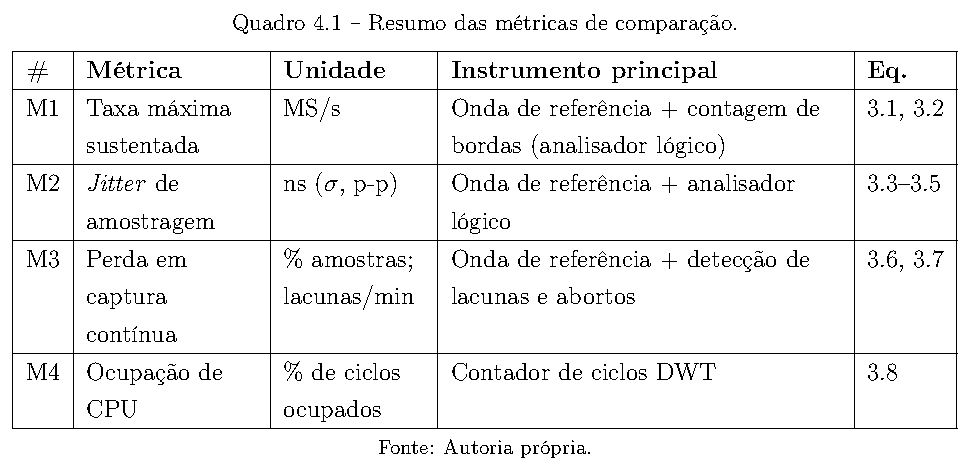
\includegraphics[width=0.94\linewidth,height=0.74\textheight,keepaspectratio]{quadro_4_1_resumo_metricas.pdf}
\end{frame}

\begin{frame}{Backup: M2, números completos (Tabela 4.3)}
  \centering
  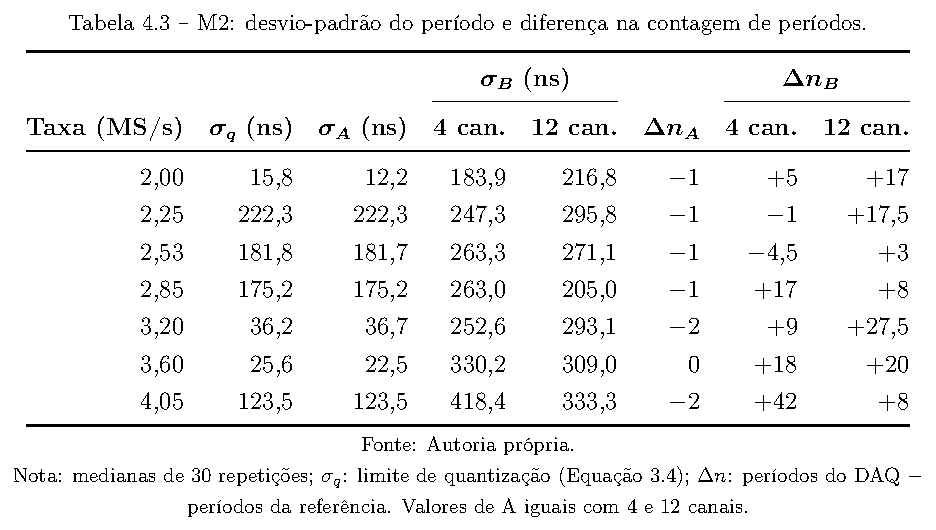
\includegraphics[width=0.94\linewidth,height=0.74\textheight,keepaspectratio]{tabela_4_3_m2_jitter.pdf}
\end{frame}

\begin{frame}{Backup: M3, números completos (Tabela 4.5)}
  \centering
  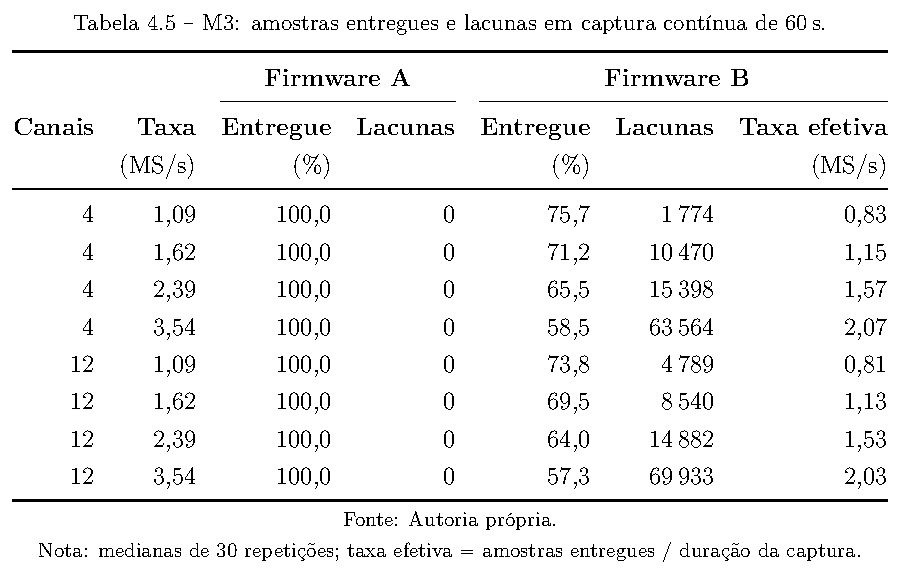
\includegraphics[width=0.90\linewidth,height=0.74\textheight,keepaspectratio]{tabela_4_5_m3_perda.pdf}
\end{frame}

\begin{frame}{Backup: M3, lacunas e capturas abortadas}
  \begin{columns}[T]
    \begin{column}{0.49\textwidth}
      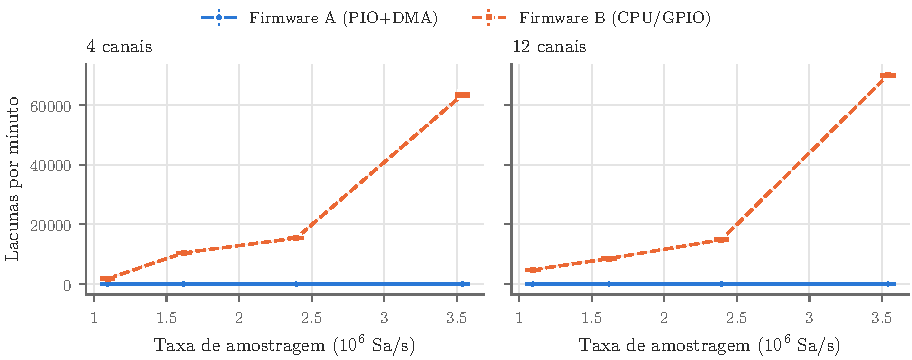
\includegraphics[width=\linewidth]{fig_4_6_m3_lacunas.pdf}
    \end{column}
    \begin{column}{0.49\textwidth}
      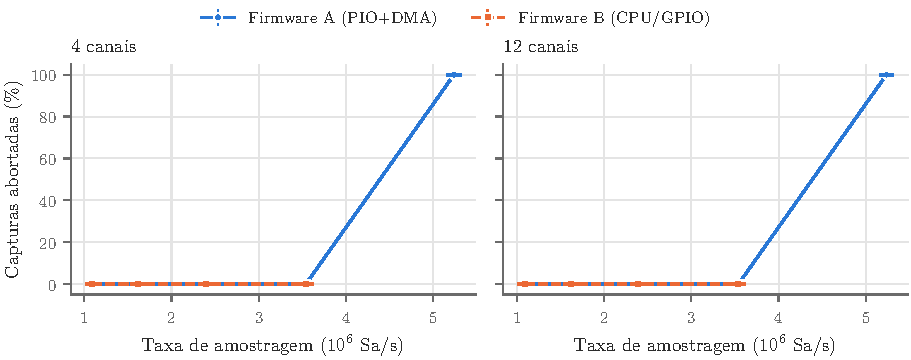
\includegraphics[width=\linewidth]{fig_4_7_m3_abortadas.pdf}
    \end{column}
  \end{columns}
  \centering\src{Autoria própria.}
\end{frame}

\begin{frame}{Backup: M3, posição das lacunas no bloco}
  \centering
  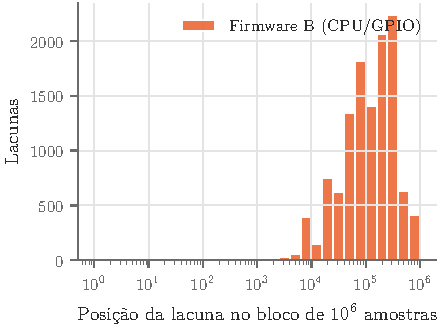
\includegraphics[height=0.58\textheight]{fig_extra_m3_posicao_lacunas.pdf}\\[2pt]
  \src{Autoria própria.}
  \vspace{2pt}
  {\footnotesize\color{ufalSlate}0,3\,\% das lacunas de B nas primeiras 20
  amostras: ligadas ao laço, não ao rearme de blocos.}
\end{frame}

\begin{frame}{Backup: síntese dos resultados (Quadro 4.2)}
  \centering
  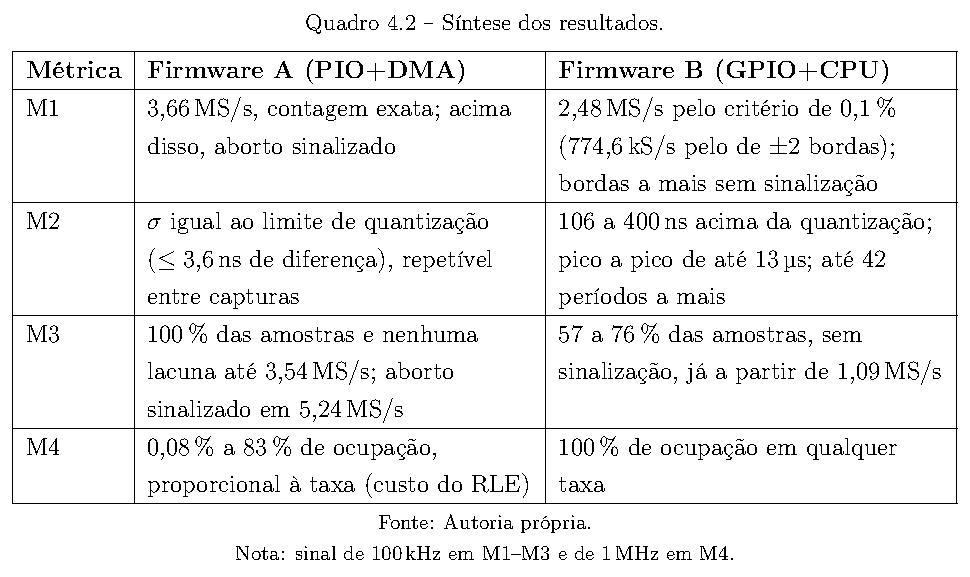
\includegraphics[width=0.94\linewidth,height=0.74\textheight,keepaspectratio]{quadro_4_2_sintese_resultados.pdf}
\end{frame}

\begin{frame}{Backup: limitações do estudo (Quadro 5.1, 1/2)}
  \centering
  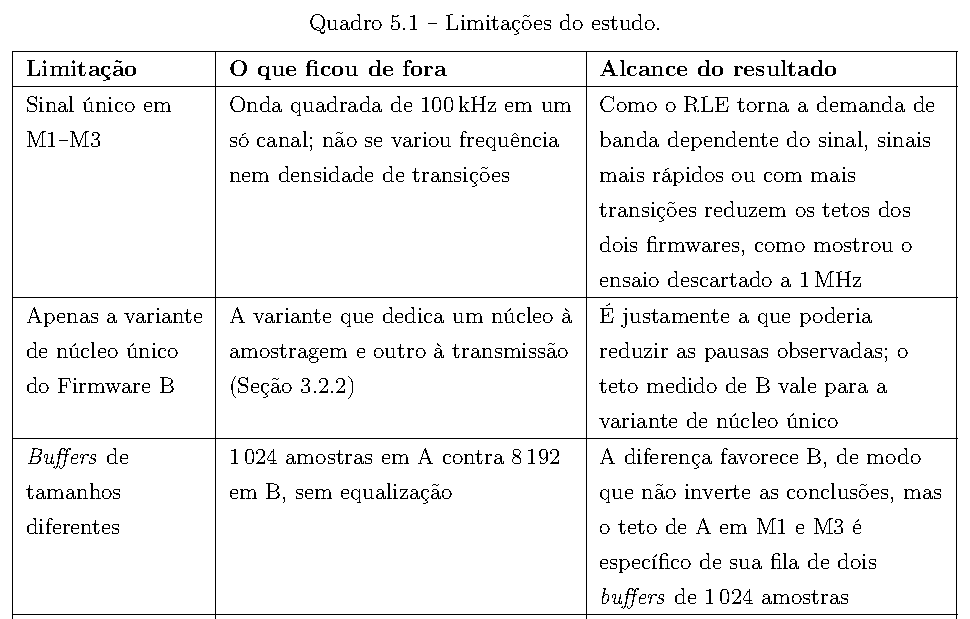
\includegraphics[width=\linewidth,height=0.76\textheight,keepaspectratio]{quadro_5_1_limitacoes_p1.pdf}
\end{frame}

\begin{frame}{Backup: limitações do estudo (Quadro 5.1, 2/2)}
  \centering
  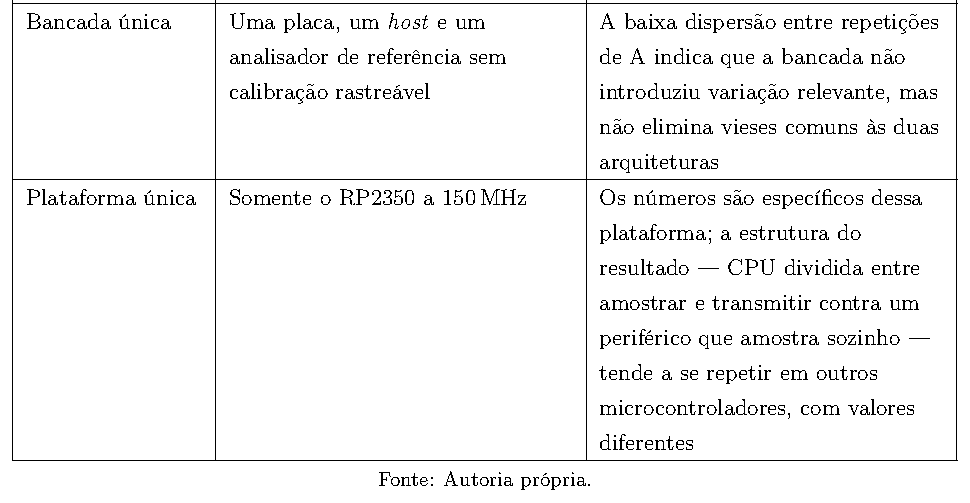
\includegraphics[width=\linewidth,height=0.76\textheight,keepaspectratio]{quadro_5_1_limitacoes_p2.pdf}
\end{frame}

\begin{frame}{Backup: trabalhos relacionados (Quadro 2.1, 1/2)}
  \centering
  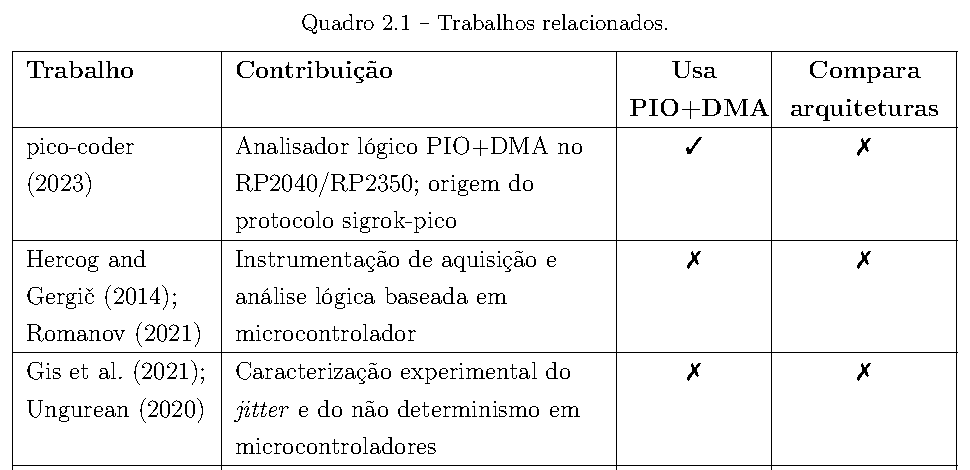
\includegraphics[width=\linewidth,height=0.76\textheight,keepaspectratio]{quadro_2_1_trabalhos_relacionados_p1.pdf}
\end{frame}

\begin{frame}{Backup: trabalhos relacionados (Quadro 2.1, 2/2)}
  \centering
  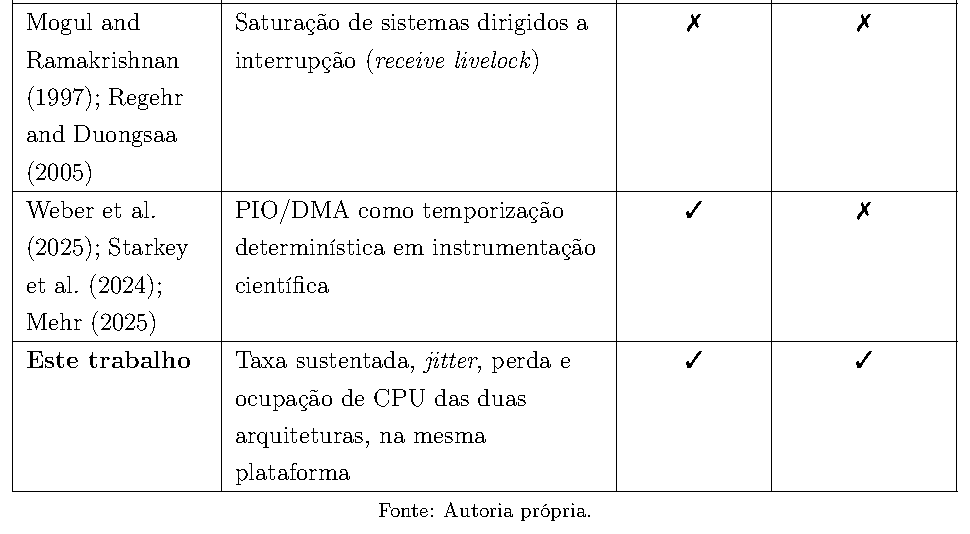
\includegraphics[width=\linewidth,height=0.76\textheight,keepaspectratio]{quadro_2_1_trabalhos_relacionados_p2.pdf}
\end{frame}

\begin{frame}{Backup: memória dos \en{firmwares} (Tabela 3.1)}
  \centering
  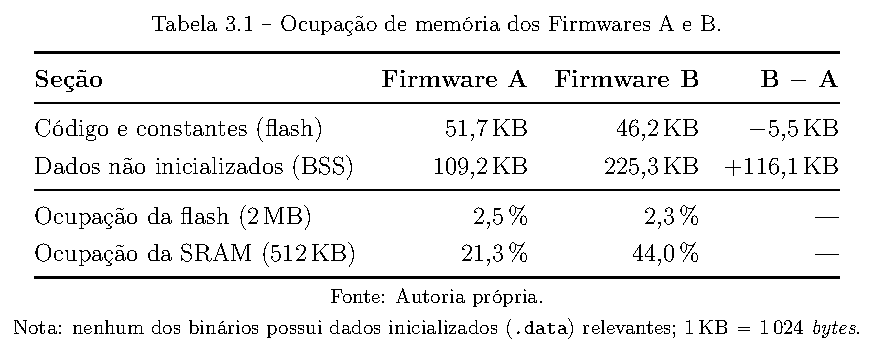
\includegraphics[width=0.80\linewidth,height=0.74\textheight,keepaspectratio]{tabela_3_1_memoria_firmwares.pdf}
\end{frame}

\begin{frame}{Backup: RP2350, \en{crossbar} e DMA}
  \begin{columns}[T]
    \begin{column}{0.49\textwidth}
      \centering
      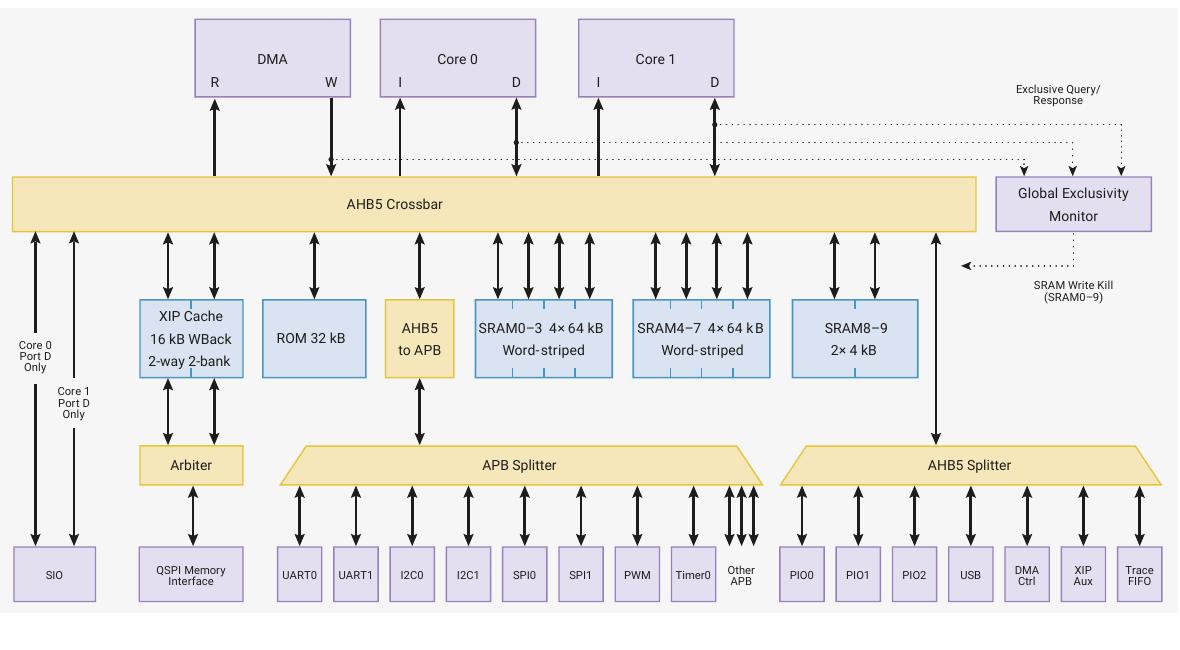
\includegraphics[width=\linewidth]{fig_2_4_crossbar_ahb5.png}\\[2pt]
      \src{Raspberry Pi Ltd., 2024.}
    \end{column}
    \begin{column}{0.49\textwidth}
      \centering
      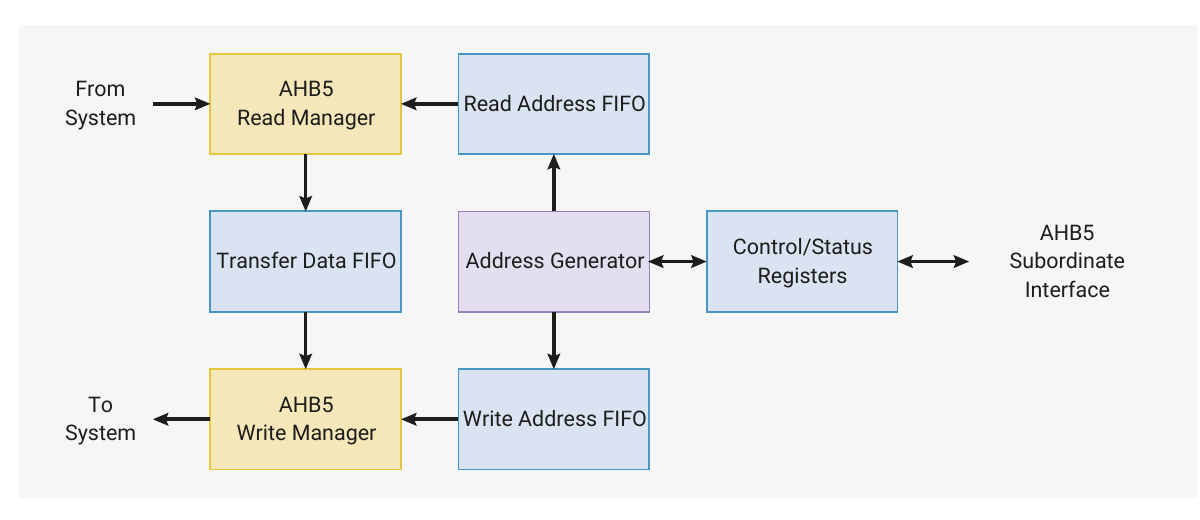
\includegraphics[width=0.86\linewidth]{fig_2_6_dma_arquitetura.png}\\[2pt]
      \src{Raspberry Pi Ltd., 2024.}
    \end{column}
  \end{columns}
  \vspace{4pt}
  {\footnotesize\color{ufalSlate}Núcleos, DMA e PIO disputam as portas de SRAM,
  XIP e APB: origem da arbitragem de barramento citada na M2.}
\end{frame}

\begin{frame}{Backup: placa e bancada física}
  \begin{columns}[T]
    \begin{column}{0.30\textwidth}
      \centering
      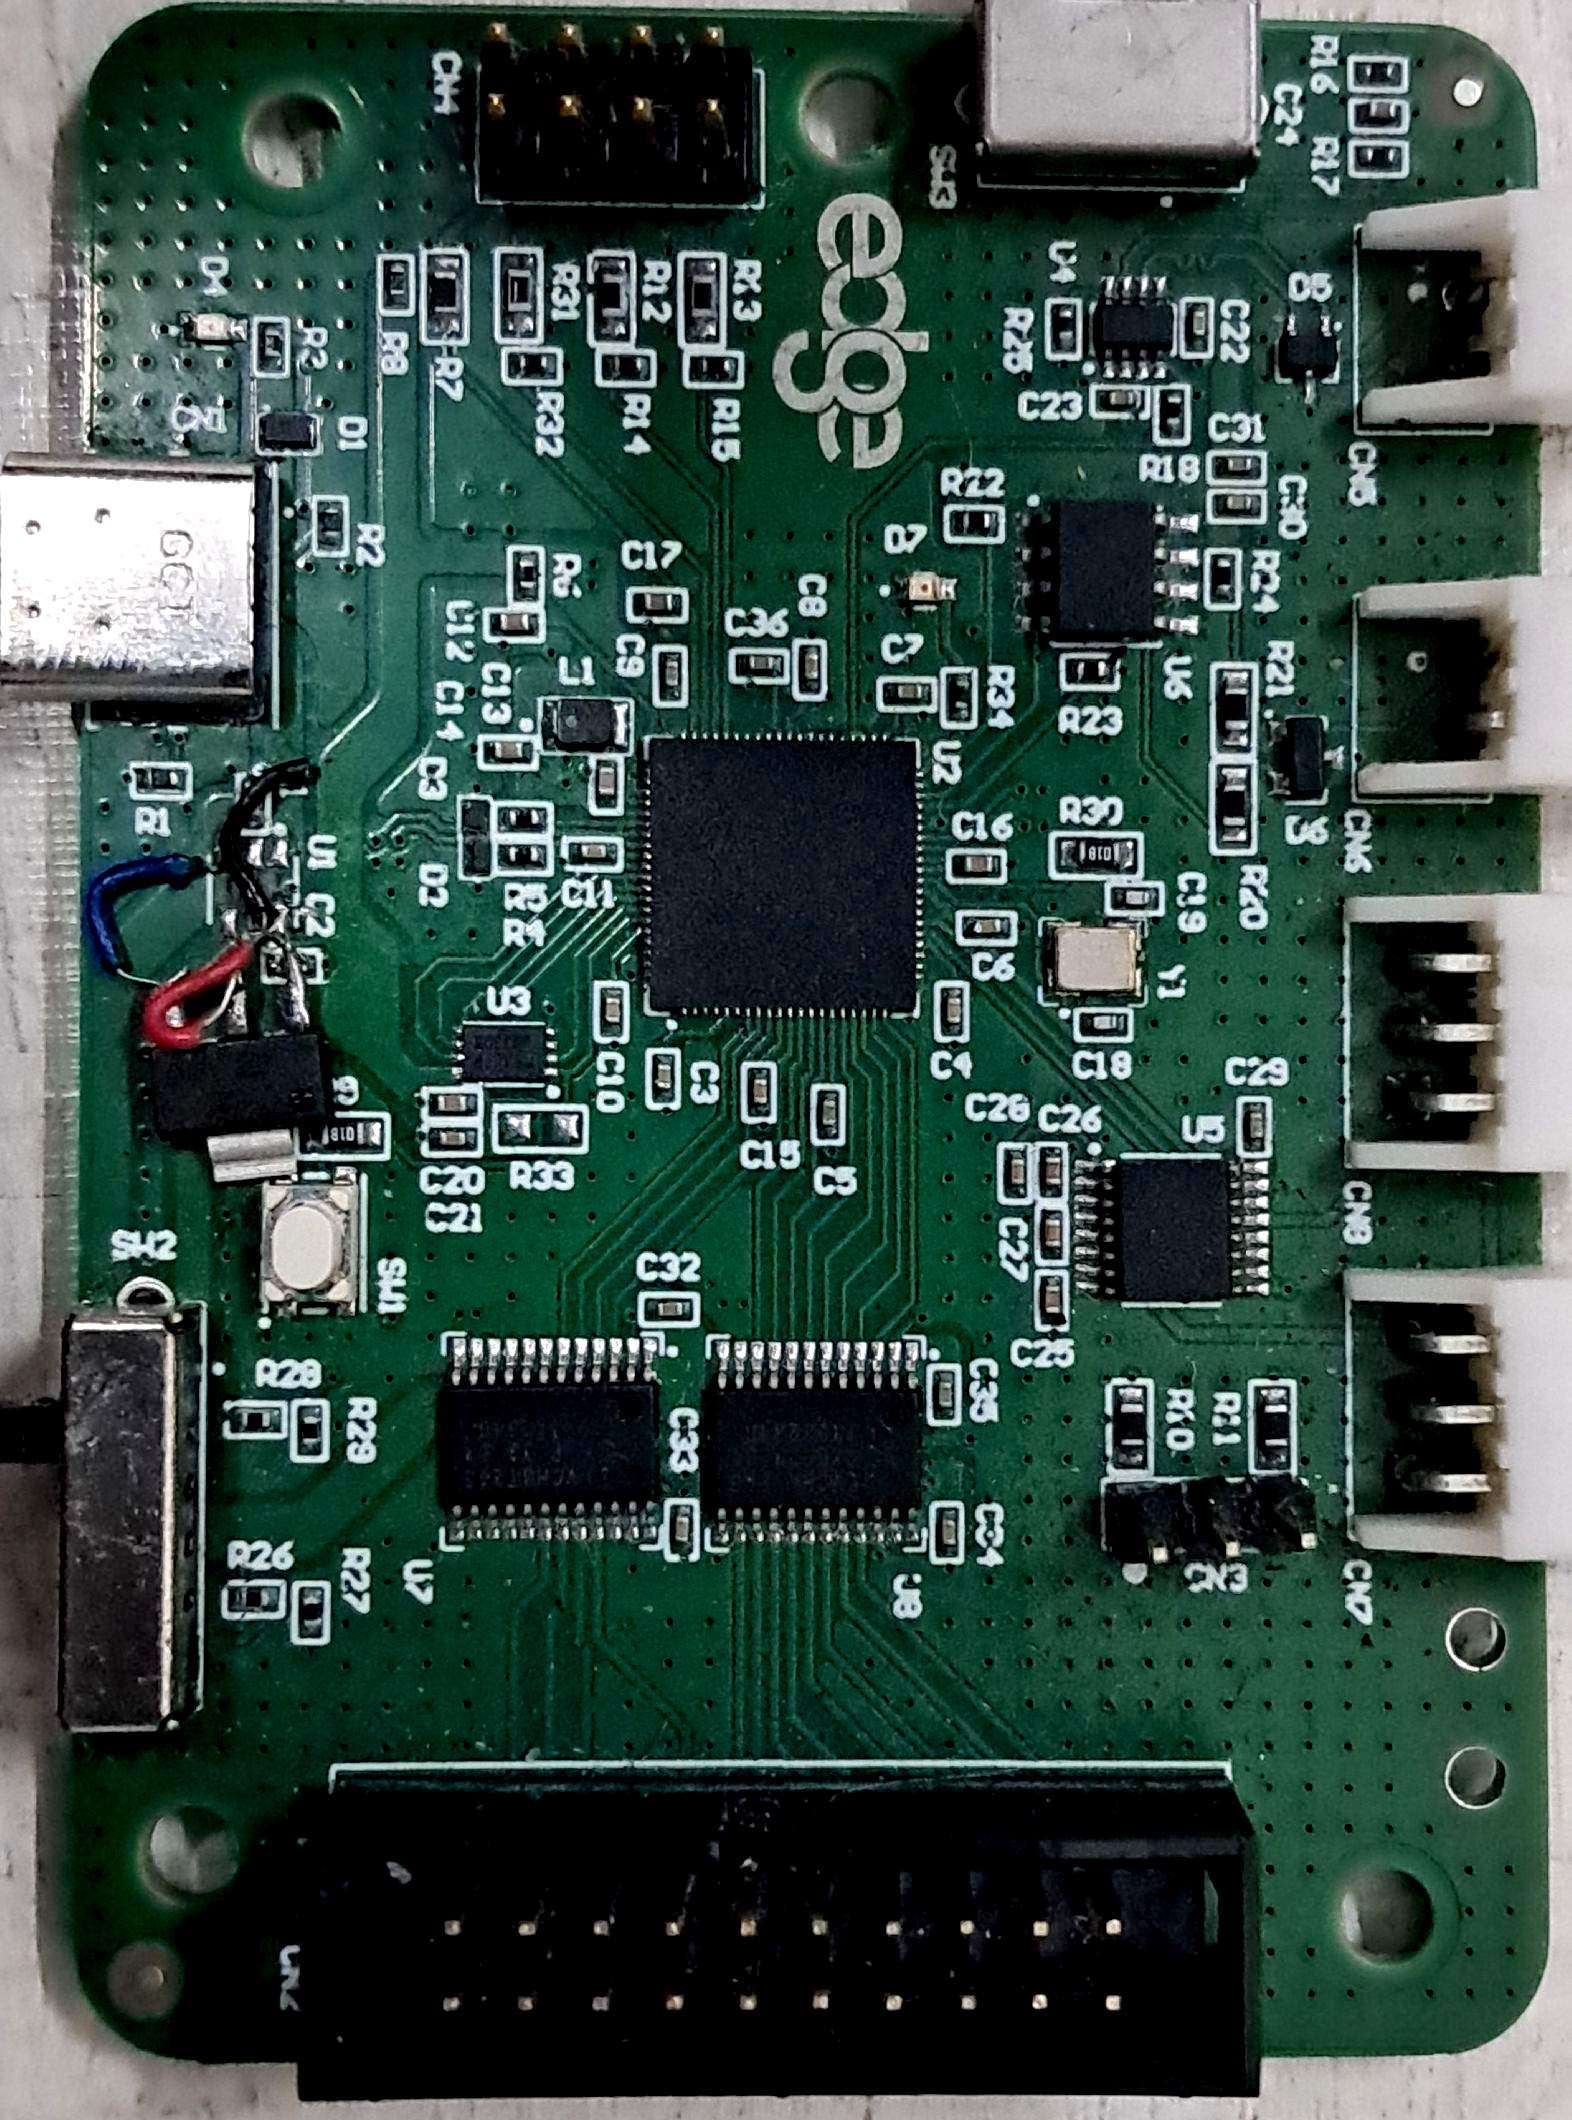
\includegraphics[height=0.62\textheight]{fig_3_2a_placa_daq_top.jpg}\\[2pt]
      \src{Autoria própria.}
    \end{column}
    \begin{column}{0.66\textwidth}
      \centering
      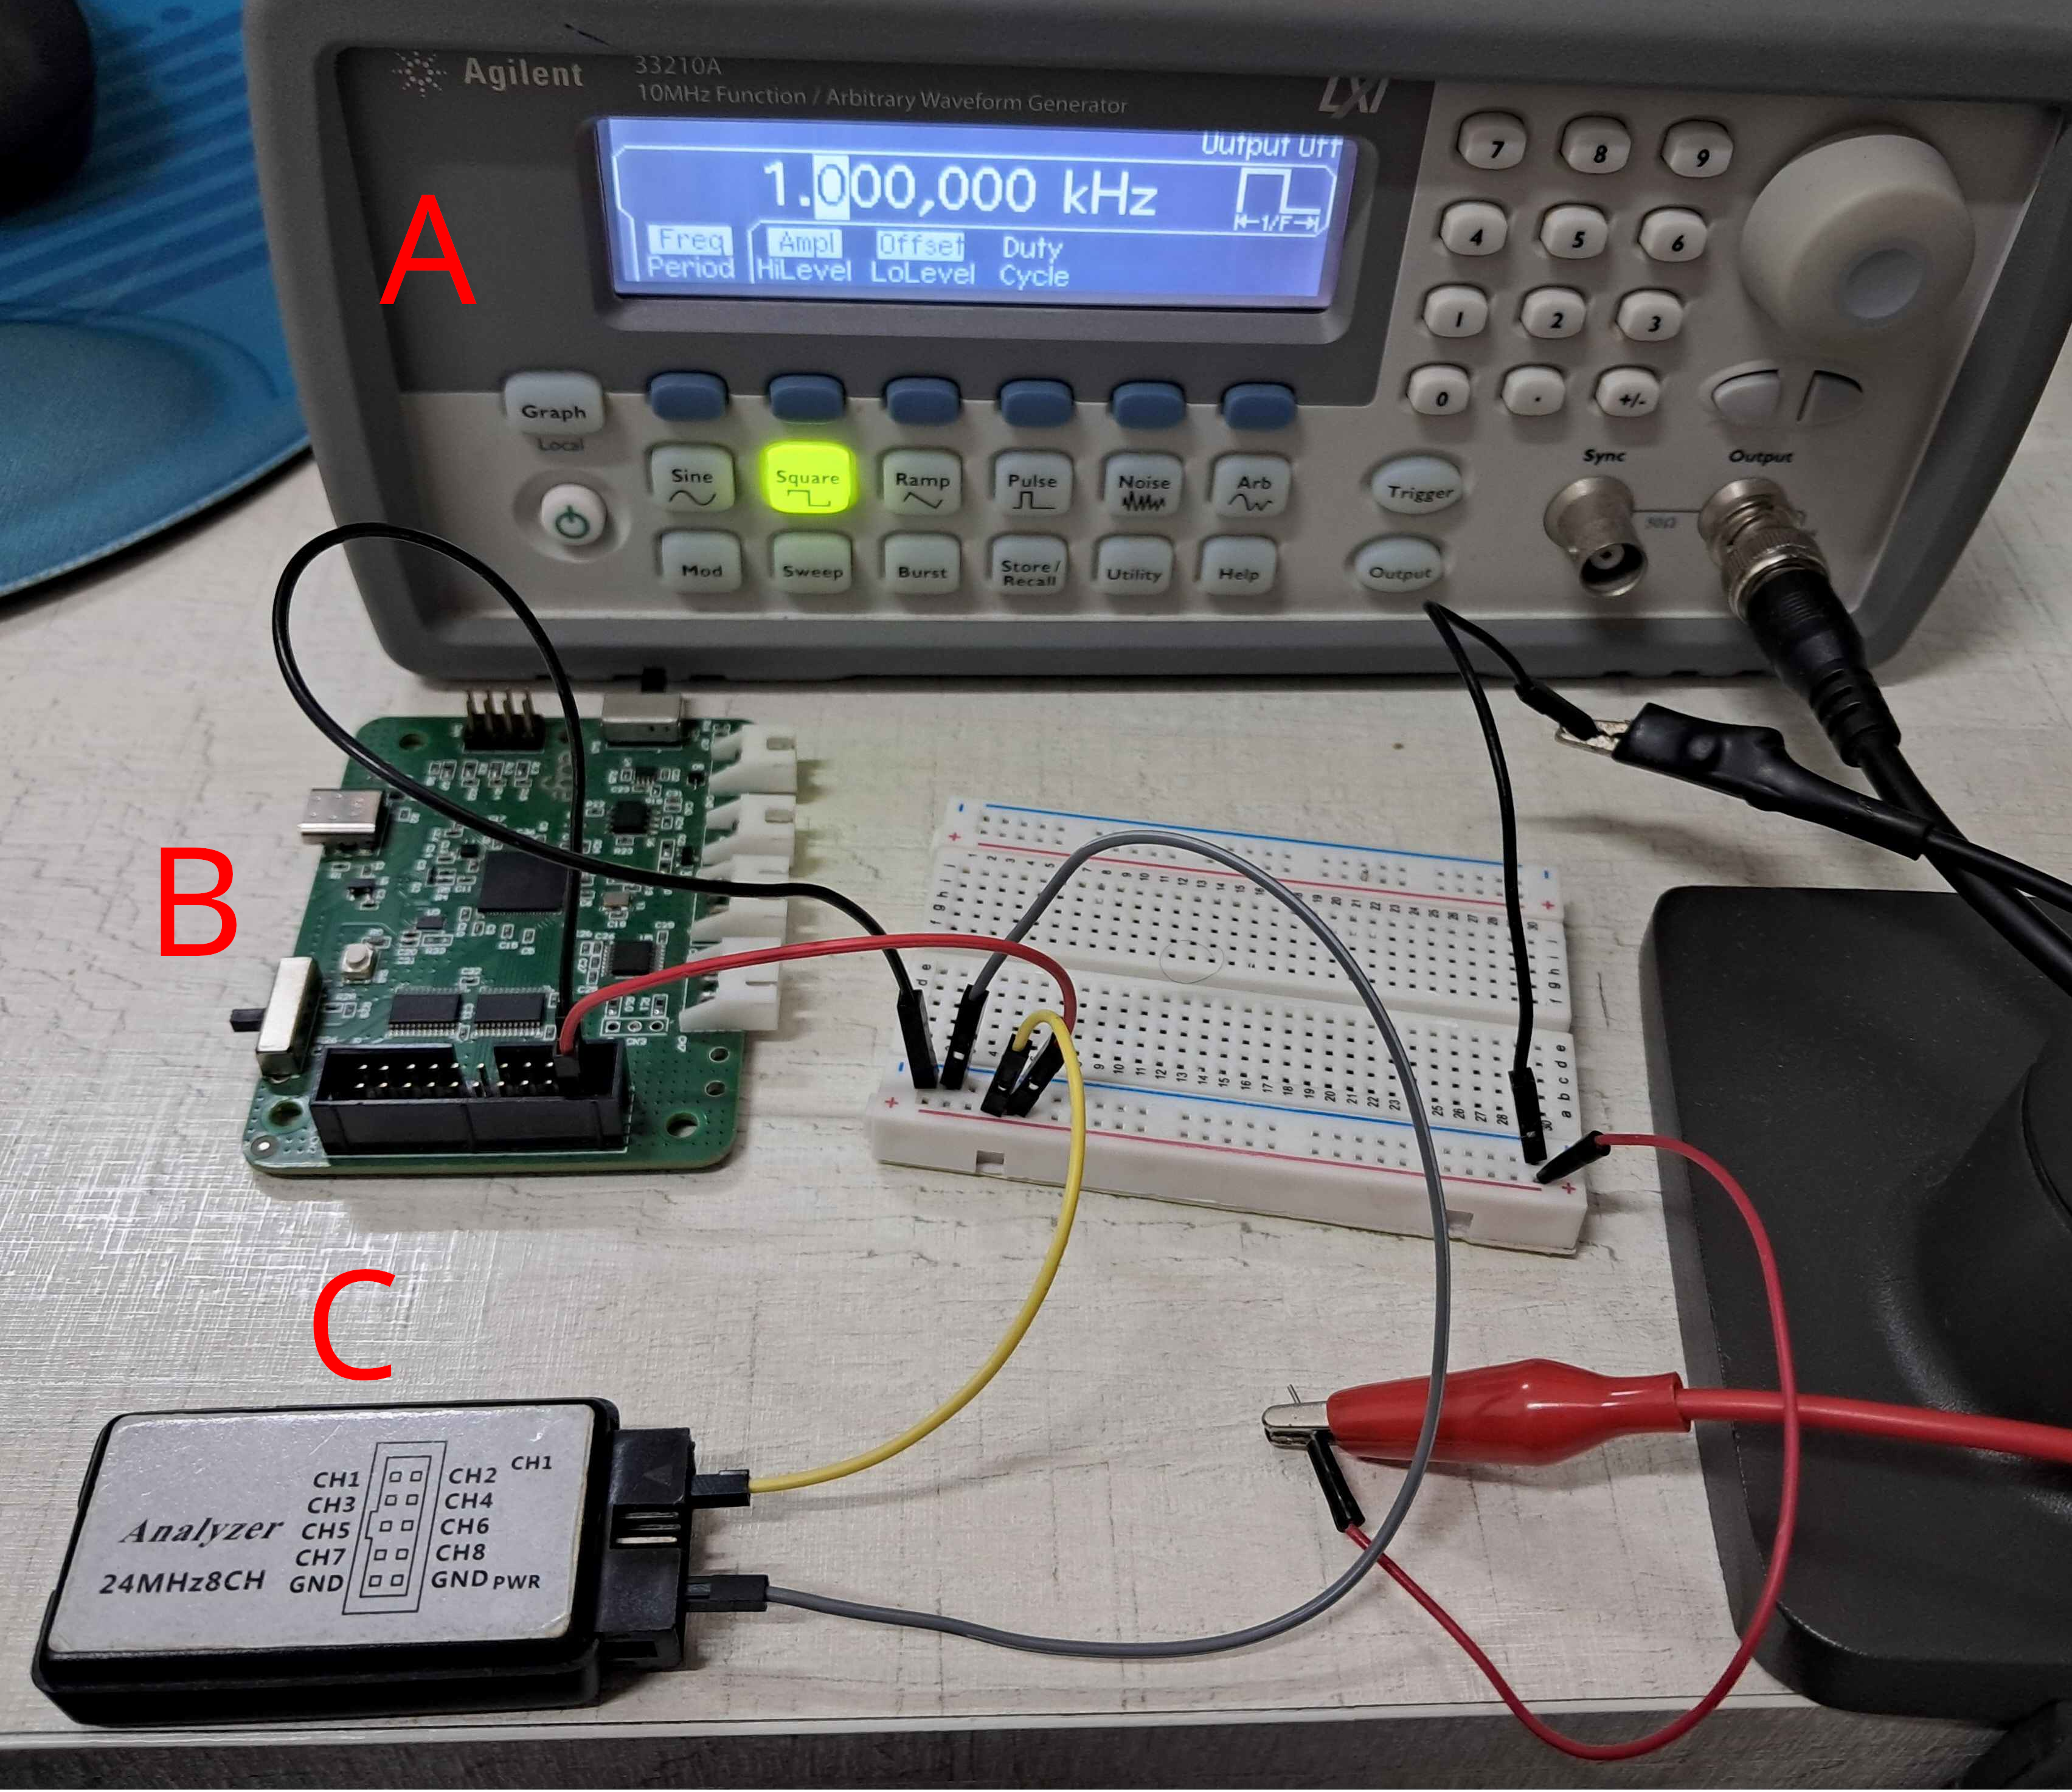
\includegraphics[height=0.62\textheight]{fig_3_1b_bancada_fisica.png}\\[2pt]
      \src{Autoria própria.}
    \end{column}
  \end{columns}
\end{frame}

\end{document}
